\documentclass[aps,10pt,prd,twocolumn,floats,letterpaper,showpacs,nofootinbib,bibnotes,notitlepage,superscriptaddress,floatfix]{revtex4-1}

\usepackage{graphicx}
\usepackage{mathrsfs}
\usepackage[intlimits,centertags]{amsmath}
\usepackage{amssymb,amsfonts}
\usepackage[pdftex]{hyperref}
\usepackage[x11names]{xcolor}
\usepackage{enumerate}
\usepackage{xfrac}
\usepackage[normalem]{ulem}
%\usepackage{subcaption}
\usepackage{float}

%\usepackage[caption=false]{subfig}

\usepackage{lineno}
\linenumbers

\hypersetup{pdftitle={IceCube Data for Neutrino Point-Source Searches: Years 2012-2018},
pdfsubject={IceCube Data for Neutrino Point-Source Searches: Years 2012-2018},
pdfauthor={IceCube Collaboration},
pdfstartview={FitH},
colorlinks=true,
bookmarksopen=false,
bookmarksnumbered=false,
bookmarksopenlevel=0,
linkcolor=Blue1!60!black,
citecolor=Green1!50!black,
urlcolor=Blue1!70!black}

\newcommand{\MA}[1]{{\color{black}#1}}

\begin{document}

\title{IceCube Data for Neutrino Point-Source Searches: Years 2008--2018}

\author{Author list in final version}
%\affiliation{III. Physikalisches Institut, RWTH Aachen University, D-52056 Aachen, Germany}
\affiliation{Department of Physics, University of Adelaide, Adelaide, 5005, Australia}
\affiliation{Dept. of Physics and Astronomy, University of Alaska Anchorage, 3211 Providence Dr., Anchorage, AK 99508, USA}
\affiliation{Dept. of Physics, University of Texas at Arlington, 502 Yates St., Science Hall Rm 108, Box 19059, Arlington, TX 76019, USA}
\affiliation{CTSPS, Clark-Atlanta University, Atlanta, GA 30314, USA}
\affiliation{School of Physics and Center for Relativistic Astrophysics, Georgia Institute of Technology, Atlanta, GA 30332, USA}
\affiliation{Dept. of Physics, Southern University, Baton Rouge, LA 70813, USA}
\affiliation{Dept. of Physics, University of California, Berkeley, CA 94720, USA}
\affiliation{Lawrence Berkeley National Laboratory, Berkeley, CA 94720, USA}
\affiliation{Institut f{\"u}r Physik, Humboldt-Universit{\"a}t zu Berlin, D-12489 Berlin, Germany}
\affiliation{Fakult{\"a}t f{\"u}r Physik {\&} Astronomie, Ruhr-Universit{\"a}t Bochum, D-44780 Bochum, Germany}
\affiliation{Universit{\'e} Libre de Bruxelles, Science Faculty CP230, B-1050 Brussels, Belgium}
\affiliation{Vrije Universiteit Brussel (VUB), Dienst ELEM, B-1050 Brussels, Belgium}
\affiliation{Department of Physics and Laboratory for Particle Physics and Cosmology, Harvard University, Cambridge, MA 02138, USA}
\affiliation{Dept. of Physics, Massachusetts Institute of Technology, Cambridge, MA 02139, USA}
\affiliation{Dept. of Physics and Institute for Global Prominent Research, Chiba University, Chiba 263-8522, Japan}
\affiliation{Department of Physics, Loyola University Chicago, Chicago, IL 60660, USA}
\affiliation{Dept. of Physics and Astronomy, University of Canterbury, Private Bag 4800, Christchurch, New Zealand}
\affiliation{Dept. of Physics, University of Maryland, College Park, MD 20742, USA}
\affiliation{Dept. of Astronomy, Ohio State University, Columbus, OH 43210, USA}
\affiliation{Dept. of Physics and Center for Cosmology and Astro-Particle Physics, Ohio State University, Columbus, OH 43210, USA}
\affiliation{Niels Bohr Institute, University of Copenhagen, DK-2100 Copenhagen, Denmark}
\affiliation{Dept. of Physics, TU Dortmund University, D-44221 Dortmund, Germany}
\affiliation{Dept. of Physics and Astronomy, Michigan State University, East Lansing, MI 48824, USA}
\affiliation{Dept. of Physics, University of Alberta, Edmonton, Alberta, Canada T6G 2E1}
\affiliation{Erlangen Centre for Astroparticle Physics, Friedrich-Alexander-Universit{\"a}t Erlangen-N{\"u}rnberg, D-91058 Erlangen, Germany}
\affiliation{Physik-department, Technische Universit{\"a}t M{\"u}nchen, D-85748 Garching, Germany}
\affiliation{D{\'e}partement de physique nucl{\'e}aire et corpusculaire, Universit{\'e} de Gen{\`e}ve, CH-1211 Gen{\`e}ve, Switzerland}
\affiliation{Dept. of Physics and Astronomy, University of Gent, B-9000 Gent, Belgium}
\affiliation{Dept. of Physics and Astronomy, University of California, Irvine, CA 92697, USA}
\affiliation{Karlsruhe Institute of Technology, Institut f{\"u}r Kernphysik, D-76021 Karlsruhe, Germany}
\affiliation{Dept. of Physics and Astronomy, University of Kansas, Lawrence, KS 66045, USA}
\affiliation{SNOLAB, 1039 Regional Road 24, Creighton Mine 9, Lively, ON, Canada P3Y 1N2}
\affiliation{Department of Physics and Astronomy, UCLA, Los Angeles, CA 90095, USA}
\affiliation{Department of Physics, Mercer University, Macon, GA 31207-0001, USA}
\affiliation{Dept. of Astronomy, University of Wisconsin{\textendash}Madison, Madison, WI 53706, USA}
\affiliation{Dept. of Physics and Wisconsin IceCube Particle Astrophysics Center, University of Wisconsin{\textendash}Madison, Madison, WI 53706, USA}
\affiliation{Institute of Physics, University of Mainz, Staudinger Weg 7, D-55099 Mainz, Germany}
\affiliation{Department of Physics, Marquette University, Milwaukee, WI, 53201, USA}
\affiliation{Institut f{\"u}r Kernphysik, Westf{\"a}lische Wilhelms-Universit{\"a}t M{\"u}nster, D-48149 M{\"u}nster, Germany}
\affiliation{Bartol Research Institute and Dept. of Physics and Astronomy, University of Delaware, Newark, DE 19716, USA}
\affiliation{Dept. of Physics, Yale University, New Haven, CT 06520, USA}
\affiliation{Dept. of Physics, University of Oxford, Parks Road, Oxford OX1 3PU, UK}
\affiliation{Dept. of Physics, Drexel University, 3141 Chestnut Street, Philadelphia, PA 19104, USA}
\affiliation{Physics Department, South Dakota School of Mines and Technology, Rapid City, SD 57701, USA}
\affiliation{Dept. of Physics, University of Wisconsin, River Falls, WI 54022, USA}
\affiliation{Dept. of Physics and Astronomy, University of Rochester, Rochester, NY 14627, USA}
\affiliation{Oskar Klein Centre and Dept. of Physics, Stockholm University, SE-10691 Stockholm, Sweden}
\affiliation{Dept. of Physics and Astronomy, Stony Brook University, Stony Brook, NY 11794-3800, USA}
\affiliation{Dept. of Physics, Sungkyunkwan University, Suwon 16419, Korea}
\affiliation{Institute of Basic Science, Sungkyunkwan University, Suwon 16419, Korea}
\affiliation{Dept. of Physics and Astronomy, University of Alabama, Tuscaloosa, AL 35487, USA}
\affiliation{Dept. of Astronomy and Astrophysics, Pennsylvania State University, University Park, PA 16802, USA}
\affiliation{Dept. of Physics, Pennsylvania State University, University Park, PA 16802, USA}
\affiliation{Dept. of Physics and Astronomy, Uppsala University, Box 516, S-75120 Uppsala, Sweden}
\affiliation{Dept. of Physics, University of Wuppertal, D-42119 Wuppertal, Germany}
\affiliation{DESY, D-15738 Zeuthen, Germany}

\author{R. Abbasi}
\affiliation{Department of Physics, Loyola University Chicago, Chicago, IL 60660, USA}
\author{M. Ackermann}
\affiliation{DESY, D-15738 Zeuthen, Germany}
\author{J. Adams}
\affiliation{Dept. of Physics and Astronomy, University of Canterbury, Private Bag 4800, Christchurch, New Zealand}
\author{J. A. Aguilar}
\affiliation{Universit{\'e} Libre de Bruxelles, Science Faculty CP230, B-1050 Brussels, Belgium}
\author{M. Ahlers}
\affiliation{Niels Bohr Institute, University of Copenhagen, DK-2100 Copenhagen, Denmark}
\author{M. Ahrens}
\affiliation{Oskar Klein Centre and Dept. of Physics, Stockholm University, SE-10691 Stockholm, Sweden}
\author{C. Alispach}
\affiliation{D{\'e}partement de physique nucl{\'e}aire et corpusculaire, Universit{\'e} de Gen{\`e}ve, CH-1211 Gen{\`e}ve, Switzerland}
\author{N. M. Amin}
\affiliation{Bartol Research Institute and Dept. of Physics and Astronomy, University of Delaware, Newark, DE 19716, USA}
\author{K. Andeen}
\affiliation{Department of Physics, Marquette University, Milwaukee, WI, 53201, USA}
\author{T. Anderson}
\affiliation{Dept. of Physics, Pennsylvania State University, University Park, PA 16802, USA}
\author{I. Ansseau}
\affiliation{Universit{\'e} Libre de Bruxelles, Science Faculty CP230, B-1050 Brussels, Belgium}
\author{G. Anton}
\affiliation{Erlangen Centre for Astroparticle Physics, Friedrich-Alexander-Universit{\"a}t Erlangen-N{\"u}rnberg, D-91058 Erlangen, Germany}
\author{C. Arg{\"u}elles}
\affiliation{Department of Physics and Laboratory for Particle Physics and Cosmology, Harvard University, Cambridge, MA 02138, USA}
\author{S. Axani}
\affiliation{Dept. of Physics, Massachusetts Institute of Technology, Cambridge, MA 02139, USA}
\author{X. Bai}
\affiliation{Physics Department, South Dakota School of Mines and Technology, Rapid City, SD 57701, USA}
\author{A. Balagopal V.}
\affiliation{Karlsruhe Institute of Technology, Institut f{\"u}r Kernphysik, D-76021 Karlsruhe, Germany}
\author{A. Barbano}
\affiliation{D{\'e}partement de physique nucl{\'e}aire et corpusculaire, Universit{\'e} de Gen{\`e}ve, CH-1211 Gen{\`e}ve, Switzerland}
\author{S. W. Barwick}
\affiliation{Dept. of Physics and Astronomy, University of California, Irvine, CA 92697, USA}
\author{B. Bastian}
\affiliation{DESY, D-15738 Zeuthen, Germany}
\author{V. Basu}
\affiliation{Dept. of Physics and Wisconsin IceCube Particle Astrophysics Center, University of Wisconsin{\textendash}Madison, Madison, WI 53706, USA}
\author{V. Baum}
\affiliation{Institute of Physics, University of Mainz, Staudinger Weg 7, D-55099 Mainz, Germany}
\author{S. Baur}
\affiliation{Universit{\'e} Libre de Bruxelles, Science Faculty CP230, B-1050 Brussels, Belgium}
\author{R. Bay}
\affiliation{Dept. of Physics, University of California, Berkeley, CA 94720, USA}
\author{J. J. Beatty}
\affiliation{Dept. of Astronomy, Ohio State University, Columbus, OH 43210, USA}
\affiliation{Dept. of Physics and Center for Cosmology and Astro-Particle Physics, Ohio State University, Columbus, OH 43210, USA}
\author{K.-H. Becker}
\affiliation{Dept. of Physics, University of Wuppertal, D-42119 Wuppertal, Germany}
\author{J. Becker Tjus}
\affiliation{Fakult{\"a}t f{\"u}r Physik {\&} Astronomie, Ruhr-Universit{\"a}t Bochum, D-44780 Bochum, Germany}
\author{C. Bellenghi}
\affiliation{Physik-department, Technische Universit{\"a}t M{\"u}nchen, D-85748 Garching, Germany}
\author{S. BenZvi}
\affiliation{Dept. of Physics and Astronomy, University of Rochester, Rochester, NY 14627, USA}
\author{D. Berley}
\affiliation{Dept. of Physics, University of Maryland, College Park, MD 20742, USA}
\author{E. Bernardini}
\thanks{also at Universit{\`a} di Padova, I-35131 Padova, Italy}
\affiliation{DESY, D-15738 Zeuthen, Germany}
\author{D. Z. Besson}
\thanks{also at National Research Nuclear University, Moscow Engineering Physics Institute (MEPhI), Moscow 115409, Russia}
\affiliation{Dept. of Physics and Astronomy, University of Kansas, Lawrence, KS 66045, USA}
\author{G. Binder}
\affiliation{Dept. of Physics, University of California, Berkeley, CA 94720, USA}
\affiliation{Lawrence Berkeley National Laboratory, Berkeley, CA 94720, USA}
\author{D. Bindig}
\affiliation{Dept. of Physics, University of Wuppertal, D-42119 Wuppertal, Germany}
\author{E. Blaufuss}
\affiliation{Dept. of Physics, University of Maryland, College Park, MD 20742, USA}
\author{S. Blot}
\affiliation{DESY, D-15738 Zeuthen, Germany}
\author{C. Bohm}
\affiliation{Oskar Klein Centre and Dept. of Physics, Stockholm University, SE-10691 Stockholm, Sweden}
\author{S. B{\"o}ser}
\affiliation{Institute of Physics, University of Mainz, Staudinger Weg 7, D-55099 Mainz, Germany}
\author{O. Botner}
\affiliation{Dept. of Physics and Astronomy, Uppsala University, Box 516, S-75120 Uppsala, Sweden}
\author{J. B{\"o}ttcher}
\affiliation{III. Physikalisches Institut, RWTH Aachen University, D-52056 Aachen, Germany}
\author{E. Bourbeau}
\affiliation{Niels Bohr Institute, University of Copenhagen, DK-2100 Copenhagen, Denmark}
\author{J. Bourbeau}
\affiliation{Dept. of Physics and Wisconsin IceCube Particle Astrophysics Center, University of Wisconsin{\textendash}Madison, Madison, WI 53706, USA}
\author{F. Bradascio}
\affiliation{DESY, D-15738 Zeuthen, Germany}
\author{J. Braun}
\affiliation{Dept. of Physics and Wisconsin IceCube Particle Astrophysics Center, University of Wisconsin{\textendash}Madison, Madison, WI 53706, USA}
\author{S. Bron}
\affiliation{D{\'e}partement de physique nucl{\'e}aire et corpusculaire, Universit{\'e} de Gen{\`e}ve, CH-1211 Gen{\`e}ve, Switzerland}
\author{J. Brostean-Kaiser}
\affiliation{DESY, D-15738 Zeuthen, Germany}
\author{A. Burgman}
\affiliation{Dept. of Physics and Astronomy, Uppsala University, Box 516, S-75120 Uppsala, Sweden}
\author{J. Buscher}
\affiliation{III. Physikalisches Institut, RWTH Aachen University, D-52056 Aachen, Germany}
\author{R. S. Busse}
\affiliation{Institut f{\"u}r Kernphysik, Westf{\"a}lische Wilhelms-Universit{\"a}t M{\"u}nster, D-48149 M{\"u}nster, Germany}
\author{M. A. Campana}
\affiliation{Dept. of Physics, Drexel University, 3141 Chestnut Street, Philadelphia, PA 19104, USA}
\author{T. Carver}
\affiliation{D{\'e}partement de physique nucl{\'e}aire et corpusculaire, Universit{\'e} de Gen{\`e}ve, CH-1211 Gen{\`e}ve, Switzerland}
\author{C. Chen}
\affiliation{School of Physics and Center for Relativistic Astrophysics, Georgia Institute of Technology, Atlanta, GA 30332, USA}
\author{E. Cheung}
\affiliation{Dept. of Physics, University of Maryland, College Park, MD 20742, USA}
\author{D. Chirkin}
\affiliation{Dept. of Physics and Wisconsin IceCube Particle Astrophysics Center, University of Wisconsin{\textendash}Madison, Madison, WI 53706, USA}
\author{S. Choi}
\affiliation{Dept. of Physics, Sungkyunkwan University, Suwon 16419, Korea}
\author{B. A. Clark}
\affiliation{Dept. of Physics and Astronomy, Michigan State University, East Lansing, MI 48824, USA}
\author{K. Clark}
\affiliation{SNOLAB, 1039 Regional Road 24, Creighton Mine 9, Lively, ON, Canada P3Y 1N2}
\author{L. Classen}
\affiliation{Institut f{\"u}r Kernphysik, Westf{\"a}lische Wilhelms-Universit{\"a}t M{\"u}nster, D-48149 M{\"u}nster, Germany}
\author{A. Coleman}
\affiliation{Bartol Research Institute and Dept. of Physics and Astronomy, University of Delaware, Newark, DE 19716, USA}
\author{G. H. Collin}
\affiliation{Dept. of Physics, Massachusetts Institute of Technology, Cambridge, MA 02139, USA}
\author{J. M. Conrad}
\affiliation{Dept. of Physics, Massachusetts Institute of Technology, Cambridge, MA 02139, USA}
\author{P. Coppin}
\affiliation{Vrije Universiteit Brussel (VUB), Dienst ELEM, B-1050 Brussels, Belgium}
\author{P. Correa}
\affiliation{Vrije Universiteit Brussel (VUB), Dienst ELEM, B-1050 Brussels, Belgium}
\author{D. F. Cowen}
\affiliation{Dept. of Astronomy and Astrophysics, Pennsylvania State University, University Park, PA 16802, USA}
\affiliation{Dept. of Physics, Pennsylvania State University, University Park, PA 16802, USA}
\author{R. Cross}
\affiliation{Dept. of Physics and Astronomy, University of Rochester, Rochester, NY 14627, USA}
\author{P. Dave}
\affiliation{School of Physics and Center for Relativistic Astrophysics, Georgia Institute of Technology, Atlanta, GA 30332, USA}
\author{C. De Clercq}
\affiliation{Vrije Universiteit Brussel (VUB), Dienst ELEM, B-1050 Brussels, Belgium}
\author{J. J. DeLaunay}
\affiliation{Dept. of Physics, Pennsylvania State University, University Park, PA 16802, USA}
\author{H. Dembinski}
\affiliation{Bartol Research Institute and Dept. of Physics and Astronomy, University of Delaware, Newark, DE 19716, USA}
\author{K. Deoskar}
\affiliation{Oskar Klein Centre and Dept. of Physics, Stockholm University, SE-10691 Stockholm, Sweden}
\author{S. De Ridder}
\affiliation{Dept. of Physics and Astronomy, University of Gent, B-9000 Gent, Belgium}
\author{A. Desai}
\affiliation{Dept. of Physics and Wisconsin IceCube Particle Astrophysics Center, University of Wisconsin{\textendash}Madison, Madison, WI 53706, USA}
\author{P. Desiati}
\affiliation{Dept. of Physics and Wisconsin IceCube Particle Astrophysics Center, University of Wisconsin{\textendash}Madison, Madison, WI 53706, USA}
\author{K. D. de Vries}
\affiliation{Vrije Universiteit Brussel (VUB), Dienst ELEM, B-1050 Brussels, Belgium}
\author{G. de Wasseige}
\affiliation{Vrije Universiteit Brussel (VUB), Dienst ELEM, B-1050 Brussels, Belgium}
\author{M. de With}
\affiliation{Institut f{\"u}r Physik, Humboldt-Universit{\"a}t zu Berlin, D-12489 Berlin, Germany}
\author{T. DeYoung}
\affiliation{Dept. of Physics and Astronomy, Michigan State University, East Lansing, MI 48824, USA}
\author{S. Dharani}
\affiliation{III. Physikalisches Institut, RWTH Aachen University, D-52056 Aachen, Germany}
\author{A. Diaz}
\affiliation{Dept. of Physics, Massachusetts Institute of Technology, Cambridge, MA 02139, USA}
\author{J. C. D{\'\i}az-V{\'e}lez}
\affiliation{Dept. of Physics and Wisconsin IceCube Particle Astrophysics Center, University of Wisconsin{\textendash}Madison, Madison, WI 53706, USA}
\author{H. Dujmovic}
\affiliation{Karlsruhe Institute of Technology, Institut f{\"u}r Kernphysik, D-76021 Karlsruhe, Germany}
\author{M. Dunkman}
\affiliation{Dept. of Physics, Pennsylvania State University, University Park, PA 16802, USA}
\author{M. A. DuVernois}
\affiliation{Dept. of Physics and Wisconsin IceCube Particle Astrophysics Center, University of Wisconsin{\textendash}Madison, Madison, WI 53706, USA}
\author{E. Dvorak}
\affiliation{Physics Department, South Dakota School of Mines and Technology, Rapid City, SD 57701, USA}
\author{T. Ehrhardt}
\affiliation{Institute of Physics, University of Mainz, Staudinger Weg 7, D-55099 Mainz, Germany}
\author{P. Eller}
\affiliation{Physik-department, Technische Universit{\"a}t M{\"u}nchen, D-85748 Garching, Germany}
\author{R. Engel}
\affiliation{Karlsruhe Institute of Technology, Institut f{\"u}r Kernphysik, D-76021 Karlsruhe, Germany}
\author{P. A. Evenson}
\affiliation{Bartol Research Institute and Dept. of Physics and Astronomy, University of Delaware, Newark, DE 19716, USA}
\author{S. Fahey}
\affiliation{Dept. of Physics and Wisconsin IceCube Particle Astrophysics Center, University of Wisconsin{\textendash}Madison, Madison, WI 53706, USA}
\author{A. R. Fazely}
\affiliation{Dept. of Physics, Southern University, Baton Rouge, LA 70813, USA}
\author{J. Felde}
\affiliation{Dept. of Physics, University of Maryland, College Park, MD 20742, USA}
\author{A.T. Fienberg}
\affiliation{Dept. of Physics, Pennsylvania State University, University Park, PA 16802, USA}
\author{K. Filimonov}
\affiliation{Dept. of Physics, University of California, Berkeley, CA 94720, USA}
\author{C. Finley}
\affiliation{Oskar Klein Centre and Dept. of Physics, Stockholm University, SE-10691 Stockholm, Sweden}
\author{L. Fischer}
\affiliation{DESY, D-15738 Zeuthen, Germany}
\author{D. Fox}
\affiliation{Dept. of Astronomy and Astrophysics, Pennsylvania State University, University Park, PA 16802, USA}
\author{A. Franckowiak}
\affiliation{DESY, D-15738 Zeuthen, Germany}
\author{E. Friedman}
\affiliation{Dept. of Physics, University of Maryland, College Park, MD 20742, USA}
\author{A. Fritz}
\affiliation{Institute of Physics, University of Mainz, Staudinger Weg 7, D-55099 Mainz, Germany}
\author{T. K. Gaisser}
\affiliation{Bartol Research Institute and Dept. of Physics and Astronomy, University of Delaware, Newark, DE 19716, USA}
\author{J. Gallagher}
\affiliation{Dept. of Astronomy, University of Wisconsin{\textendash}Madison, Madison, WI 53706, USA}
\author{E. Ganster}
\affiliation{III. Physikalisches Institut, RWTH Aachen University, D-52056 Aachen, Germany}
\author{S. Garrappa}
\affiliation{DESY, D-15738 Zeuthen, Germany}
\author{L. Gerhardt}
\affiliation{Lawrence Berkeley National Laboratory, Berkeley, CA 94720, USA}
\author{A. Ghadimi}
\affiliation{Dept. of Physics and Astronomy, University of Alabama, Tuscaloosa, AL 35487, USA}
\author{T. Glauch}
\affiliation{Physik-department, Technische Universit{\"a}t M{\"u}nchen, D-85748 Garching, Germany}
\author{T. Gl{\"u}senkamp}
\affiliation{Erlangen Centre for Astroparticle Physics, Friedrich-Alexander-Universit{\"a}t Erlangen-N{\"u}rnberg, D-91058 Erlangen, Germany}
\author{A. Goldschmidt}
\affiliation{Lawrence Berkeley National Laboratory, Berkeley, CA 94720, USA}
\author{J. G. Gonzalez}
\affiliation{Bartol Research Institute and Dept. of Physics and Astronomy, University of Delaware, Newark, DE 19716, USA}
\author{S. Goswami}
\affiliation{Dept. of Physics and Astronomy, University of Alabama, Tuscaloosa, AL 35487, USA}
\author{D. Grant}
\affiliation{Dept. of Physics and Astronomy, Michigan State University, East Lansing, MI 48824, USA}
\author{T. Gr{\'e}goire}
\affiliation{Dept. of Physics, Pennsylvania State University, University Park, PA 16802, USA}
\author{Z. Griffith}
\affiliation{Dept. of Physics and Wisconsin IceCube Particle Astrophysics Center, University of Wisconsin{\textendash}Madison, Madison, WI 53706, USA}
\author{S. Griswold}
\affiliation{Dept. of Physics and Astronomy, University of Rochester, Rochester, NY 14627, USA}
\author{M. G{\"u}nd{\"u}z}
\affiliation{Fakult{\"a}t f{\"u}r Physik {\&} Astronomie, Ruhr-Universit{\"a}t Bochum, D-44780 Bochum, Germany}
\author{C. Haack}
\affiliation{Physik-department, Technische Universit{\"a}t M{\"u}nchen, D-85748 Garching, Germany}
\author{A. Hallgren}
\affiliation{Dept. of Physics and Astronomy, Uppsala University, Box 516, S-75120 Uppsala, Sweden}
\author{R. Halliday}
\affiliation{Dept. of Physics and Astronomy, Michigan State University, East Lansing, MI 48824, USA}
\author{L. Halve}
\affiliation{III. Physikalisches Institut, RWTH Aachen University, D-52056 Aachen, Germany}
\author{F. Halzen}
\affiliation{Dept. of Physics and Wisconsin IceCube Particle Astrophysics Center, University of Wisconsin{\textendash}Madison, Madison, WI 53706, USA}
\author{M. Ha Minh}
\affiliation{Physik-department, Technische Universit{\"a}t M{\"u}nchen, D-85748 Garching, Germany}
\author{K. Hanson}
\affiliation{Dept. of Physics and Wisconsin IceCube Particle Astrophysics Center, University of Wisconsin{\textendash}Madison, Madison, WI 53706, USA}
\author{J. Hardin}
\affiliation{Dept. of Physics and Wisconsin IceCube Particle Astrophysics Center, University of Wisconsin{\textendash}Madison, Madison, WI 53706, USA}
\author{A. Haungs}
\affiliation{Karlsruhe Institute of Technology, Institut f{\"u}r Kernphysik, D-76021 Karlsruhe, Germany}
\author{S. Hauser}
\affiliation{III. Physikalisches Institut, RWTH Aachen University, D-52056 Aachen, Germany}
\author{D. Hebecker}
\affiliation{Institut f{\"u}r Physik, Humboldt-Universit{\"a}t zu Berlin, D-12489 Berlin, Germany}
\author{P. Heix}
\affiliation{III. Physikalisches Institut, RWTH Aachen University, D-52056 Aachen, Germany}
\author{K. Helbing}
\affiliation{Dept. of Physics, University of Wuppertal, D-42119 Wuppertal, Germany}
\author{R. Hellauer}
\affiliation{Dept. of Physics, University of Maryland, College Park, MD 20742, USA}
\author{F. Henningsen}
\affiliation{Physik-department, Technische Universit{\"a}t M{\"u}nchen, D-85748 Garching, Germany}
\author{S. Hickford}
\affiliation{Dept. of Physics, University of Wuppertal, D-42119 Wuppertal, Germany}
\author{J. Hignight}
\affiliation{Dept. of Physics, University of Alberta, Edmonton, Alberta, Canada T6G 2E1}
\author{C. Hill}
\affiliation{Dept. of Physics and Institute for Global Prominent Research, Chiba University, Chiba 263-8522, Japan}
\author{G. C. Hill}
\affiliation{Department of Physics, University of Adelaide, Adelaide, 5005, Australia}
\author{K. D. Hoffman}
\affiliation{Dept. of Physics, University of Maryland, College Park, MD 20742, USA}
\author{R. Hoffmann}
\affiliation{Dept. of Physics, University of Wuppertal, D-42119 Wuppertal, Germany}
\author{T. Hoinka}
\affiliation{Dept. of Physics, TU Dortmund University, D-44221 Dortmund, Germany}
\author{B. Hokanson-Fasig}
\affiliation{Dept. of Physics and Wisconsin IceCube Particle Astrophysics Center, University of Wisconsin{\textendash}Madison, Madison, WI 53706, USA}
\author{K. Hoshina}
\thanks{also at Earthquake Research Institute, University of Tokyo, Bunkyo, Tokyo 113-0032, Japan}
\affiliation{Dept. of Physics and Wisconsin IceCube Particle Astrophysics Center, University of Wisconsin{\textendash}Madison, Madison, WI 53706, USA}
\author{F. Huang}
\affiliation{Dept. of Physics, Pennsylvania State University, University Park, PA 16802, USA}
\author{M. Huber}
\affiliation{Physik-department, Technische Universit{\"a}t M{\"u}nchen, D-85748 Garching, Germany}
\author{T. Huber}
\affiliation{Karlsruhe Institute of Technology, Institut f{\"u}r Kernphysik, D-76021 Karlsruhe, Germany}
\author{K. Hultqvist}
\affiliation{Oskar Klein Centre and Dept. of Physics, Stockholm University, SE-10691 Stockholm, Sweden}
\author{M. H{\"u}nnefeld}
\affiliation{Dept. of Physics, TU Dortmund University, D-44221 Dortmund, Germany}
\author{R. Hussain}
\affiliation{Dept. of Physics and Wisconsin IceCube Particle Astrophysics Center, University of Wisconsin{\textendash}Madison, Madison, WI 53706, USA}
\author{S. In}
\affiliation{Dept. of Physics, Sungkyunkwan University, Suwon 16419, Korea}
\author{N. Iovine}
\affiliation{Universit{\'e} Libre de Bruxelles, Science Faculty CP230, B-1050 Brussels, Belgium}
\author{A. Ishihara}
\affiliation{Dept. of Physics and Institute for Global Prominent Research, Chiba University, Chiba 263-8522, Japan}
\author{M. Jansson}
\affiliation{Oskar Klein Centre and Dept. of Physics, Stockholm University, SE-10691 Stockholm, Sweden}
\author{G. S. Japaridze}
\affiliation{CTSPS, Clark-Atlanta University, Atlanta, GA 30314, USA}
\author{M. Jeong}
\affiliation{Dept. of Physics, Sungkyunkwan University, Suwon 16419, Korea}
\author{B. J. P. Jones}
\affiliation{Dept. of Physics, University of Texas at Arlington, 502 Yates St., Science Hall Rm 108, Box 19059, Arlington, TX 76019, USA}
\author{F. Jonske}
\affiliation{III. Physikalisches Institut, RWTH Aachen University, D-52056 Aachen, Germany}
\author{R. Joppe}
\affiliation{III. Physikalisches Institut, RWTH Aachen University, D-52056 Aachen, Germany}
\author{D. Kang}
\affiliation{Karlsruhe Institute of Technology, Institut f{\"u}r Kernphysik, D-76021 Karlsruhe, Germany}
\author{W. Kang}
\affiliation{Dept. of Physics, Sungkyunkwan University, Suwon 16419, Korea}
\author{X. Kang}
\affiliation{Dept. of Physics, Drexel University, 3141 Chestnut Street, Philadelphia, PA 19104, USA}
\author{A. Kappes}
\affiliation{Institut f{\"u}r Kernphysik, Westf{\"a}lische Wilhelms-Universit{\"a}t M{\"u}nster, D-48149 M{\"u}nster, Germany}
\author{D. Kappesser}
\affiliation{Institute of Physics, University of Mainz, Staudinger Weg 7, D-55099 Mainz, Germany}
\author{T. Karg}
\affiliation{DESY, D-15738 Zeuthen, Germany}
\author{M. Karl}
\affiliation{Physik-department, Technische Universit{\"a}t M{\"u}nchen, D-85748 Garching, Germany}
\author{A. Karle}
\affiliation{Dept. of Physics and Wisconsin IceCube Particle Astrophysics Center, University of Wisconsin{\textendash}Madison, Madison, WI 53706, USA}
\author{U. Katz}
\affiliation{Erlangen Centre for Astroparticle Physics, Friedrich-Alexander-Universit{\"a}t Erlangen-N{\"u}rnberg, D-91058 Erlangen, Germany}
\author{M. Kauer}
\affiliation{Dept. of Physics and Wisconsin IceCube Particle Astrophysics Center, University of Wisconsin{\textendash}Madison, Madison, WI 53706, USA}
\author{M. Kellermann}
\affiliation{III. Physikalisches Institut, RWTH Aachen University, D-52056 Aachen, Germany}
\author{J. L. Kelley}
\affiliation{Dept. of Physics and Wisconsin IceCube Particle Astrophysics Center, University of Wisconsin{\textendash}Madison, Madison, WI 53706, USA}
\author{A. Kheirandish}
\affiliation{Dept. of Physics, Pennsylvania State University, University Park, PA 16802, USA}
\author{J. Kim}
\affiliation{Dept. of Physics, Sungkyunkwan University, Suwon 16419, Korea}
\author{K. Kin}
\affiliation{Dept. of Physics and Institute for Global Prominent Research, Chiba University, Chiba 263-8522, Japan}
\author{T. Kintscher}
\affiliation{DESY, D-15738 Zeuthen, Germany}
\author{J. Kiryluk}
\affiliation{Dept. of Physics and Astronomy, Stony Brook University, Stony Brook, NY 11794-3800, USA}
\author{T. Kittler}
\affiliation{Erlangen Centre for Astroparticle Physics, Friedrich-Alexander-Universit{\"a}t Erlangen-N{\"u}rnberg, D-91058 Erlangen, Germany}
\author{S. R. Klein}
\affiliation{Dept. of Physics, University of California, Berkeley, CA 94720, USA}
\affiliation{Lawrence Berkeley National Laboratory, Berkeley, CA 94720, USA}
\author{R. Koirala}
\affiliation{Bartol Research Institute and Dept. of Physics and Astronomy, University of Delaware, Newark, DE 19716, USA}
\author{H. Kolanoski}
\affiliation{Institut f{\"u}r Physik, Humboldt-Universit{\"a}t zu Berlin, D-12489 Berlin, Germany}
\author{L. K{\"o}pke}
\affiliation{Institute of Physics, University of Mainz, Staudinger Weg 7, D-55099 Mainz, Germany}
\author{C. Kopper}
\affiliation{Dept. of Physics and Astronomy, Michigan State University, East Lansing, MI 48824, USA}
\author{S. Kopper}
\affiliation{Dept. of Physics and Astronomy, University of Alabama, Tuscaloosa, AL 35487, USA}
\author{D. J. Koskinen}
\affiliation{Niels Bohr Institute, University of Copenhagen, DK-2100 Copenhagen, Denmark}
\author{P. Koundal}
\affiliation{Karlsruhe Institute of Technology, Institut f{\"u}r Kernphysik, D-76021 Karlsruhe, Germany}
\author{M. Kovacevich}
\affiliation{Dept. of Physics, Drexel University, 3141 Chestnut Street, Philadelphia, PA 19104, USA}
\author{M. Kowalski}
\affiliation{Institut f{\"u}r Physik, Humboldt-Universit{\"a}t zu Berlin, D-12489 Berlin, Germany}
\affiliation{DESY, D-15738 Zeuthen, Germany}
\author{K. Krings}
\affiliation{Physik-department, Technische Universit{\"a}t M{\"u}nchen, D-85748 Garching, Germany}
\author{G. Kr{\"u}ckl}
\affiliation{Institute of Physics, University of Mainz, Staudinger Weg 7, D-55099 Mainz, Germany}
\author{N. Kulacz}
\affiliation{Dept. of Physics, University of Alberta, Edmonton, Alberta, Canada T6G 2E1}
\author{N. Kurahashi}
\affiliation{Dept. of Physics, Drexel University, 3141 Chestnut Street, Philadelphia, PA 19104, USA}
\author{A. Kyriacou}
\affiliation{Department of Physics, University of Adelaide, Adelaide, 5005, Australia}
\author{C. Lagunas Gualda}
\affiliation{DESY, D-15738 Zeuthen, Germany}
\author{J. L. Lanfranchi}
\affiliation{Dept. of Physics, Pennsylvania State University, University Park, PA 16802, USA}
\author{M. J. Larson}
\affiliation{Dept. of Physics, University of Maryland, College Park, MD 20742, USA}
\author{F. Lauber}
\affiliation{Dept. of Physics, University of Wuppertal, D-42119 Wuppertal, Germany}
\author{J. P. Lazar}
\affiliation{Department of Physics and Laboratory for Particle Physics and Cosmology, Harvard University, Cambridge, MA 02138, USA}
\affiliation{Dept. of Physics and Wisconsin IceCube Particle Astrophysics Center, University of Wisconsin{\textendash}Madison, Madison, WI 53706, USA}
\author{K. Leonard}
\affiliation{Dept. of Physics and Wisconsin IceCube Particle Astrophysics Center, University of Wisconsin{\textendash}Madison, Madison, WI 53706, USA}
\author{A. Leszczy{\'n}ska}
\affiliation{Karlsruhe Institute of Technology, Institut f{\"u}r Kernphysik, D-76021 Karlsruhe, Germany}
\author{Y. Li}
\affiliation{Dept. of Physics, Pennsylvania State University, University Park, PA 16802, USA}
\author{Q. R. Liu}
\affiliation{Dept. of Physics and Wisconsin IceCube Particle Astrophysics Center, University of Wisconsin{\textendash}Madison, Madison, WI 53706, USA}
\author{E. Lohfink}
\affiliation{Institute of Physics, University of Mainz, Staudinger Weg 7, D-55099 Mainz, Germany}
\author{C. J. Lozano Mariscal}
\affiliation{Institut f{\"u}r Kernphysik, Westf{\"a}lische Wilhelms-Universit{\"a}t M{\"u}nster, D-48149 M{\"u}nster, Germany}
\author{L. Lu}
\affiliation{Dept. of Physics and Institute for Global Prominent Research, Chiba University, Chiba 263-8522, Japan}
\author{F. Lucarelli}
\affiliation{D{\'e}partement de physique nucl{\'e}aire et corpusculaire, Universit{\'e} de Gen{\`e}ve, CH-1211 Gen{\`e}ve, Switzerland}
\author{A. Ludwig}
\affiliation{Department of Physics and Astronomy, UCLA, Los Angeles, CA 90095, USA}
\author{J. L{\"u}nemann}
\affiliation{Vrije Universiteit Brussel (VUB), Dienst ELEM, B-1050 Brussels, Belgium}
\author{W. Luszczak}
\affiliation{Dept. of Physics and Wisconsin IceCube Particle Astrophysics Center, University of Wisconsin{\textendash}Madison, Madison, WI 53706, USA}
\author{Y. Lyu}
\affiliation{Dept. of Physics, University of California, Berkeley, CA 94720, USA}
\affiliation{Lawrence Berkeley National Laboratory, Berkeley, CA 94720, USA}
\author{W. Y. Ma}
\affiliation{DESY, D-15738 Zeuthen, Germany}
\author{J. Madsen}
\affiliation{Dept. of Physics, University of Wisconsin, River Falls, WI 54022, USA}
\author{G. Maggi}
\affiliation{Vrije Universiteit Brussel (VUB), Dienst ELEM, B-1050 Brussels, Belgium}
\author{K. B. M. Mahn}
\affiliation{Dept. of Physics and Astronomy, Michigan State University, East Lansing, MI 48824, USA}
\author{Y. Makino}
\affiliation{Dept. of Physics and Wisconsin IceCube Particle Astrophysics Center, University of Wisconsin{\textendash}Madison, Madison, WI 53706, USA}
\author{P. Mallik}
\affiliation{III. Physikalisches Institut, RWTH Aachen University, D-52056 Aachen, Germany}
\author{S. Mancina}
\affiliation{Dept. of Physics and Wisconsin IceCube Particle Astrophysics Center, University of Wisconsin{\textendash}Madison, Madison, WI 53706, USA}
\author{I. C. Mari{\c{s}}}
\affiliation{Universit{\'e} Libre de Bruxelles, Science Faculty CP230, B-1050 Brussels, Belgium}
\author{R. Maruyama}
\affiliation{Dept. of Physics, Yale University, New Haven, CT 06520, USA}
\author{K. Mase}
\affiliation{Dept. of Physics and Institute for Global Prominent Research, Chiba University, Chiba 263-8522, Japan}
\author{R. Maunu}
\affiliation{Dept. of Physics, University of Maryland, College Park, MD 20742, USA}
\author{F. McNally}
\affiliation{Department of Physics, Mercer University, Macon, GA 31207-0001, USA}
\author{K. Meagher}
\affiliation{Dept. of Physics and Wisconsin IceCube Particle Astrophysics Center, University of Wisconsin{\textendash}Madison, Madison, WI 53706, USA}
\author{A. Medina}
\affiliation{Dept. of Physics and Center for Cosmology and Astro-Particle Physics, Ohio State University, Columbus, OH 43210, USA}
\author{M. Meier}
\affiliation{Dept. of Physics and Institute for Global Prominent Research, Chiba University, Chiba 263-8522, Japan}
\author{S. Meighen-Berger}
\affiliation{Physik-department, Technische Universit{\"a}t M{\"u}nchen, D-85748 Garching, Germany}
\author{J. Merz}
\affiliation{III. Physikalisches Institut, RWTH Aachen University, D-52056 Aachen, Germany}
\author{J. Micallef}
\affiliation{Dept. of Physics and Astronomy, Michigan State University, East Lansing, MI 48824, USA}
\author{D. Mockler}
\affiliation{Universit{\'e} Libre de Bruxelles, Science Faculty CP230, B-1050 Brussels, Belgium}
\author{G. Moment{\'e}}
\affiliation{Institute of Physics, University of Mainz, Staudinger Weg 7, D-55099 Mainz, Germany}
\author{T. Montaruli}
\affiliation{D{\'e}partement de physique nucl{\'e}aire et corpusculaire, Universit{\'e} de Gen{\`e}ve, CH-1211 Gen{\`e}ve, Switzerland}
\author{R. W. Moore}
\affiliation{Dept. of Physics, University of Alberta, Edmonton, Alberta, Canada T6G 2E1}
\author{R. Morse}
\affiliation{Dept. of Physics and Wisconsin IceCube Particle Astrophysics Center, University of Wisconsin{\textendash}Madison, Madison, WI 53706, USA}
\author{M. Moulai}
\affiliation{Dept. of Physics, Massachusetts Institute of Technology, Cambridge, MA 02139, USA}
\author{P. Muth}
\affiliation{III. Physikalisches Institut, RWTH Aachen University, D-52056 Aachen, Germany}
\author{R. Naab}
\affiliation{DESY, D-15738 Zeuthen, Germany}
\author{R. Nagai}
\affiliation{Dept. of Physics and Institute for Global Prominent Research, Chiba University, Chiba 263-8522, Japan}
\author{U. Naumann}
\affiliation{Dept. of Physics, University of Wuppertal, D-42119 Wuppertal, Germany}
\author{J. Necker}
\affiliation{DESY, D-15738 Zeuthen, Germany}
\author{G. Neer}
\affiliation{Dept. of Physics and Astronomy, Michigan State University, East Lansing, MI 48824, USA}
\author{L. V. Nguy{\~{\^{{e}}}}n}
\affiliation{Dept. of Physics and Astronomy, Michigan State University, East Lansing, MI 48824, USA}
\author{H. Niederhausen}
\affiliation{Physik-department, Technische Universit{\"a}t M{\"u}nchen, D-85748 Garching, Germany}
\author{M. U. Nisa}
\affiliation{Dept. of Physics and Astronomy, Michigan State University, East Lansing, MI 48824, USA}
\author{S. C. Nowicki}
\affiliation{Dept. of Physics and Astronomy, Michigan State University, East Lansing, MI 48824, USA}
\author{D. R. Nygren}
\affiliation{Lawrence Berkeley National Laboratory, Berkeley, CA 94720, USA}
\author{A. Obertacke Pollmann}
\affiliation{Dept. of Physics, University of Wuppertal, D-42119 Wuppertal, Germany}
\author{M. Oehler}
\affiliation{Karlsruhe Institute of Technology, Institut f{\"u}r Kernphysik, D-76021 Karlsruhe, Germany}
\author{A. Olivas}
\affiliation{Dept. of Physics, University of Maryland, College Park, MD 20742, USA}
\author{E. O'Sullivan}
\affiliation{Dept. of Physics and Astronomy, Uppsala University, Box 516, S-75120 Uppsala, Sweden}
\author{H. Pandya}
\affiliation{Bartol Research Institute and Dept. of Physics and Astronomy, University of Delaware, Newark, DE 19716, USA}
\author{D. V. Pankova}
\affiliation{Dept. of Physics, Pennsylvania State University, University Park, PA 16802, USA}
\author{N. Park}
\affiliation{Dept. of Physics and Wisconsin IceCube Particle Astrophysics Center, University of Wisconsin{\textendash}Madison, Madison, WI 53706, USA}
\author{G. K. Parker}
\affiliation{Dept. of Physics, University of Texas at Arlington, 502 Yates St., Science Hall Rm 108, Box 19059, Arlington, TX 76019, USA}
\author{E. N. Paudel}
\affiliation{Bartol Research Institute and Dept. of Physics and Astronomy, University of Delaware, Newark, DE 19716, USA}
\author{P. Peiffer}
\affiliation{Institute of Physics, University of Mainz, Staudinger Weg 7, D-55099 Mainz, Germany}
\author{C. P{\'e}rez de los Heros}
\affiliation{Dept. of Physics and Astronomy, Uppsala University, Box 516, S-75120 Uppsala, Sweden}
\author{S. Philippen}
\affiliation{III. Physikalisches Institut, RWTH Aachen University, D-52056 Aachen, Germany}
\author{D. Pieloth}
\affiliation{Dept. of Physics, TU Dortmund University, D-44221 Dortmund, Germany}
\author{S. Pieper}
\affiliation{Dept. of Physics, University of Wuppertal, D-42119 Wuppertal, Germany}
\author{A. Pizzuto}
\affiliation{Dept. of Physics and Wisconsin IceCube Particle Astrophysics Center, University of Wisconsin{\textendash}Madison, Madison, WI 53706, USA}
\author{M. Plum}
\affiliation{Department of Physics, Marquette University, Milwaukee, WI, 53201, USA}
\author{Y. Popovych}
\affiliation{III. Physikalisches Institut, RWTH Aachen University, D-52056 Aachen, Germany}
\author{A. Porcelli}
\affiliation{Dept. of Physics and Astronomy, University of Gent, B-9000 Gent, Belgium}
\author{M. Prado Rodriguez}
\affiliation{Dept. of Physics and Wisconsin IceCube Particle Astrophysics Center, University of Wisconsin{\textendash}Madison, Madison, WI 53706, USA}
\author{P. B. Price}
\affiliation{Dept. of Physics, University of California, Berkeley, CA 94720, USA}
\author{G. T. Przybylski}
\affiliation{Lawrence Berkeley National Laboratory, Berkeley, CA 94720, USA}
\author{C. Raab}
\affiliation{Universit{\'e} Libre de Bruxelles, Science Faculty CP230, B-1050 Brussels, Belgium}
\author{A. Raissi}
\affiliation{Dept. of Physics and Astronomy, University of Canterbury, Private Bag 4800, Christchurch, New Zealand}
\author{M. Rameez}
\affiliation{Niels Bohr Institute, University of Copenhagen, DK-2100 Copenhagen, Denmark}
\author{K. Rawlins}
\affiliation{Dept. of Physics and Astronomy, University of Alaska Anchorage, 3211 Providence Dr., Anchorage, AK 99508, USA}
\author{I. C. Rea}
\affiliation{Physik-department, Technische Universit{\"a}t M{\"u}nchen, D-85748 Garching, Germany}
\author{A. Rehman}
\affiliation{Bartol Research Institute and Dept. of Physics and Astronomy, University of Delaware, Newark, DE 19716, USA}
\author{R. Reimann}
\affiliation{III. Physikalisches Institut, RWTH Aachen University, D-52056 Aachen, Germany}
\author{M. Renschler}
\affiliation{Karlsruhe Institute of Technology, Institut f{\"u}r Kernphysik, D-76021 Karlsruhe, Germany}
\author{G. Renzi}
\affiliation{Universit{\'e} Libre de Bruxelles, Science Faculty CP230, B-1050 Brussels, Belgium}
\author{E. Resconi}
\affiliation{Physik-department, Technische Universit{\"a}t M{\"u}nchen, D-85748 Garching, Germany}
\author{S. Reusch}
\affiliation{DESY, D-15738 Zeuthen, Germany}
\author{W. Rhode}
\affiliation{Dept. of Physics, TU Dortmund University, D-44221 Dortmund, Germany}
\author{M. Richman}
\affiliation{Dept. of Physics, Drexel University, 3141 Chestnut Street, Philadelphia, PA 19104, USA}
\author{B. Riedel}
\affiliation{Dept. of Physics and Wisconsin IceCube Particle Astrophysics Center, University of Wisconsin{\textendash}Madison, Madison, WI 53706, USA}
\author{S. Robertson}
\affiliation{Dept. of Physics, University of California, Berkeley, CA 94720, USA}
\affiliation{Lawrence Berkeley National Laboratory, Berkeley, CA 94720, USA}
\author{G. Roellinghoff}
\affiliation{Dept. of Physics, Sungkyunkwan University, Suwon 16419, Korea}
\author{M. Rongen}
\affiliation{III. Physikalisches Institut, RWTH Aachen University, D-52056 Aachen, Germany}
\author{C. Rott}
\affiliation{Dept. of Physics, Sungkyunkwan University, Suwon 16419, Korea}
\author{T. Ruhe}
\affiliation{Dept. of Physics, TU Dortmund University, D-44221 Dortmund, Germany}
\author{D. Ryckbosch}
\affiliation{Dept. of Physics and Astronomy, University of Gent, B-9000 Gent, Belgium}
\author{D. Rysewyk Cantu}
\affiliation{Dept. of Physics and Astronomy, Michigan State University, East Lansing, MI 48824, USA}
\author{I. Safa}
\affiliation{Department of Physics and Laboratory for Particle Physics and Cosmology, Harvard University, Cambridge, MA 02138, USA}
\affiliation{Dept. of Physics and Wisconsin IceCube Particle Astrophysics Center, University of Wisconsin{\textendash}Madison, Madison, WI 53706, USA}
\author{S. E. Sanchez Herrera}
\affiliation{Dept. of Physics and Astronomy, Michigan State University, East Lansing, MI 48824, USA}
\author{A. Sandrock}
\affiliation{Dept. of Physics, TU Dortmund University, D-44221 Dortmund, Germany}
\author{J. Sandroos}
\affiliation{Institute of Physics, University of Mainz, Staudinger Weg 7, D-55099 Mainz, Germany}
\author{M. Santander}
\affiliation{Dept. of Physics and Astronomy, University of Alabama, Tuscaloosa, AL 35487, USA}
\author{S. Sarkar}
\affiliation{Dept. of Physics, University of Oxford, Parks Road, Oxford OX1 3PU, UK}
\author{S. Sarkar}
\affiliation{Dept. of Physics, University of Alberta, Edmonton, Alberta, Canada T6G 2E1}
\author{K. Satalecka}
\affiliation{DESY, D-15738 Zeuthen, Germany}
\author{M. Scharf}
\affiliation{III. Physikalisches Institut, RWTH Aachen University, D-52056 Aachen, Germany}
\author{M. Schaufel}
\affiliation{III. Physikalisches Institut, RWTH Aachen University, D-52056 Aachen, Germany}
\author{H. Schieler}
\affiliation{Karlsruhe Institute of Technology, Institut f{\"u}r Kernphysik, D-76021 Karlsruhe, Germany}
\author{P. Schlunder}
\affiliation{Dept. of Physics, TU Dortmund University, D-44221 Dortmund, Germany}
\author{T. Schmidt}
\affiliation{Dept. of Physics, University of Maryland, College Park, MD 20742, USA}
\author{A. Schneider}
\affiliation{Dept. of Physics and Wisconsin IceCube Particle Astrophysics Center, University of Wisconsin{\textendash}Madison, Madison, WI 53706, USA}
\author{J. Schneider}
\affiliation{Erlangen Centre for Astroparticle Physics, Friedrich-Alexander-Universit{\"a}t Erlangen-N{\"u}rnberg, D-91058 Erlangen, Germany}
\author{F. G. Schr{\"o}der}
\affiliation{Karlsruhe Institute of Technology, Institut f{\"u}r Kernphysik, D-76021 Karlsruhe, Germany}
\affiliation{Bartol Research Institute and Dept. of Physics and Astronomy, University of Delaware, Newark, DE 19716, USA}
\author{L. Schumacher}
\affiliation{III. Physikalisches Institut, RWTH Aachen University, D-52056 Aachen, Germany}
\author{S. Sclafani}
\affiliation{Dept. of Physics, Drexel University, 3141 Chestnut Street, Philadelphia, PA 19104, USA}
\author{D. Seckel}
\affiliation{Bartol Research Institute and Dept. of Physics and Astronomy, University of Delaware, Newark, DE 19716, USA}
\author{S. Seunarine}
\affiliation{Dept. of Physics, University of Wisconsin, River Falls, WI 54022, USA}
\author{S. Shefali}
\affiliation{III. Physikalisches Institut, RWTH Aachen University, D-52056 Aachen, Germany}
\author{M. Silva}
\affiliation{Dept. of Physics and Wisconsin IceCube Particle Astrophysics Center, University of Wisconsin{\textendash}Madison, Madison, WI 53706, USA}
\author{B. Smithers}
\affiliation{Dept. of Physics, University of Texas at Arlington, 502 Yates St., Science Hall Rm 108, Box 19059, Arlington, TX 76019, USA}
\author{R. Snihur}
\affiliation{Dept. of Physics and Wisconsin IceCube Particle Astrophysics Center, University of Wisconsin{\textendash}Madison, Madison, WI 53706, USA}
\author{J. Soedingrekso}
\affiliation{Dept. of Physics, TU Dortmund University, D-44221 Dortmund, Germany}
\author{D. Soldin}
\affiliation{Bartol Research Institute and Dept. of Physics and Astronomy, University of Delaware, Newark, DE 19716, USA}
\author{M. Song}
\affiliation{Dept. of Physics, University of Maryland, College Park, MD 20742, USA}
\author{G. M. Spiczak}
\affiliation{Dept. of Physics, University of Wisconsin, River Falls, WI 54022, USA}
\author{C. Spiering}
\thanks{also at National Research Nuclear University, Moscow Engineering Physics Institute (MEPhI), Moscow 115409, Russia}
\affiliation{DESY, D-15738 Zeuthen, Germany}
\author{J. Stachurska}
\affiliation{DESY, D-15738 Zeuthen, Germany}
\author{M. Stamatikos}
\affiliation{Dept. of Physics and Center for Cosmology and Astro-Particle Physics, Ohio State University, Columbus, OH 43210, USA}
\author{T. Stanev}
\affiliation{Bartol Research Institute and Dept. of Physics and Astronomy, University of Delaware, Newark, DE 19716, USA}
\author{R. Stein}
\affiliation{DESY, D-15738 Zeuthen, Germany}
\author{J. Stettner}
\affiliation{III. Physikalisches Institut, RWTH Aachen University, D-52056 Aachen, Germany}
\author{A. Steuer}
\affiliation{Institute of Physics, University of Mainz, Staudinger Weg 7, D-55099 Mainz, Germany}
\author{T. Stezelberger}
\affiliation{Lawrence Berkeley National Laboratory, Berkeley, CA 94720, USA}
\author{R. G. Stokstad}
\affiliation{Lawrence Berkeley National Laboratory, Berkeley, CA 94720, USA}
\author{N. L. Strotjohann}
\affiliation{DESY, D-15738 Zeuthen, Germany}
\author{T. St{\"u}rwald}
\affiliation{III. Physikalisches Institut, RWTH Aachen University, D-52056 Aachen, Germany}
\author{T. Stuttard}
\affiliation{Niels Bohr Institute, University of Copenhagen, DK-2100 Copenhagen, Denmark}
\author{G. W. Sullivan}
\affiliation{Dept. of Physics, University of Maryland, College Park, MD 20742, USA}
\author{I. Taboada}
\affiliation{School of Physics and Center for Relativistic Astrophysics, Georgia Institute of Technology, Atlanta, GA 30332, USA}
\author{F. Tenholt}
\affiliation{Fakult{\"a}t f{\"u}r Physik {\&} Astronomie, Ruhr-Universit{\"a}t Bochum, D-44780 Bochum, Germany}
\author{S. Ter-Antonyan}
\affiliation{Dept. of Physics, Southern University, Baton Rouge, LA 70813, USA}
\author{S. Tilav}
\affiliation{Bartol Research Institute and Dept. of Physics and Astronomy, University of Delaware, Newark, DE 19716, USA}
\author{K. Tollefson}
\affiliation{Dept. of Physics and Astronomy, Michigan State University, East Lansing, MI 48824, USA}
\author{L. Tomankova}
\affiliation{Fakult{\"a}t f{\"u}r Physik {\&} Astronomie, Ruhr-Universit{\"a}t Bochum, D-44780 Bochum, Germany}
\author{C. T{\"o}nnis}
\affiliation{Institute of Basic Science, Sungkyunkwan University, Suwon 16419, Korea}
\author{S. Toscano}
\affiliation{Universit{\'e} Libre de Bruxelles, Science Faculty CP230, B-1050 Brussels, Belgium}
\author{D. Tosi}
\affiliation{Dept. of Physics and Wisconsin IceCube Particle Astrophysics Center, University of Wisconsin{\textendash}Madison, Madison, WI 53706, USA}
\author{A. Trettin}
\affiliation{DESY, D-15738 Zeuthen, Germany}
\author{M. Tselengidou}
\affiliation{Erlangen Centre for Astroparticle Physics, Friedrich-Alexander-Universit{\"a}t Erlangen-N{\"u}rnberg, D-91058 Erlangen, Germany}
\author{C. F. Tung}
\affiliation{School of Physics and Center for Relativistic Astrophysics, Georgia Institute of Technology, Atlanta, GA 30332, USA}
\author{A. Turcati}
\affiliation{Physik-department, Technische Universit{\"a}t M{\"u}nchen, D-85748 Garching, Germany}
\author{R. Turcotte}
\affiliation{Karlsruhe Institute of Technology, Institut f{\"u}r Kernphysik, D-76021 Karlsruhe, Germany}
\author{C. F. Turley}
\affiliation{Dept. of Physics, Pennsylvania State University, University Park, PA 16802, USA}
\author{J. P. Twagirayezu}
\affiliation{Dept. of Physics and Astronomy, Michigan State University, East Lansing, MI 48824, USA}
\author{B. Ty}
\affiliation{Dept. of Physics and Wisconsin IceCube Particle Astrophysics Center, University of Wisconsin{\textendash}Madison, Madison, WI 53706, USA}
\author{E. Unger}
\affiliation{Dept. of Physics and Astronomy, Uppsala University, Box 516, S-75120 Uppsala, Sweden}
\author{M. A. Unland Elorrieta}
\affiliation{Institut f{\"u}r Kernphysik, Westf{\"a}lische Wilhelms-Universit{\"a}t M{\"u}nster, D-48149 M{\"u}nster, Germany}
\author{J. Vandenbroucke}
\affiliation{Dept. of Physics and Wisconsin IceCube Particle Astrophysics Center, University of Wisconsin{\textendash}Madison, Madison, WI 53706, USA}
\author{D. van Eijk}
\affiliation{Dept. of Physics and Wisconsin IceCube Particle Astrophysics Center, University of Wisconsin{\textendash}Madison, Madison, WI 53706, USA}
\author{N. van Eijndhoven}
\affiliation{Vrije Universiteit Brussel (VUB), Dienst ELEM, B-1050 Brussels, Belgium}
\author{D. Vannerom}
\affiliation{Dept. of Physics, Massachusetts Institute of Technology, Cambridge, MA 02139, USA}
\author{J. van Santen}
\affiliation{DESY, D-15738 Zeuthen, Germany}
\author{S. Verpoest}
\affiliation{Dept. of Physics and Astronomy, University of Gent, B-9000 Gent, Belgium}
\author{M. Vraeghe}
\affiliation{Dept. of Physics and Astronomy, University of Gent, B-9000 Gent, Belgium}
\author{C. Walck}
\affiliation{Oskar Klein Centre and Dept. of Physics, Stockholm University, SE-10691 Stockholm, Sweden}
\author{A. Wallace}
\affiliation{Department of Physics, University of Adelaide, Adelaide, 5005, Australia}
\author{T. B. Watson}
\affiliation{Dept. of Physics, University of Texas at Arlington, 502 Yates St., Science Hall Rm 108, Box 19059, Arlington, TX 76019, USA}
\author{C. Weaver}
\affiliation{Dept. of Physics, University of Alberta, Edmonton, Alberta, Canada T6G 2E1}
\author{A. Weindl}
\affiliation{Karlsruhe Institute of Technology, Institut f{\"u}r Kernphysik, D-76021 Karlsruhe, Germany}
\author{M. J. Weiss}
\affiliation{Dept. of Physics, Pennsylvania State University, University Park, PA 16802, USA}
\author{J. Weldert}
\affiliation{Institute of Physics, University of Mainz, Staudinger Weg 7, D-55099 Mainz, Germany}
\author{C. Wendt}
\affiliation{Dept. of Physics and Wisconsin IceCube Particle Astrophysics Center, University of Wisconsin{\textendash}Madison, Madison, WI 53706, USA}
\author{J. Werthebach}
\affiliation{Dept. of Physics, TU Dortmund University, D-44221 Dortmund, Germany}
\author{B. J. Whelan}
\affiliation{Department of Physics, University of Adelaide, Adelaide, 5005, Australia}
\author{N. Whitehorn}
\affiliation{Department of Physics and Astronomy, UCLA, Los Angeles, CA 90095, USA}
\author{K. Wiebe}
\affiliation{Institute of Physics, University of Mainz, Staudinger Weg 7, D-55099 Mainz, Germany}
\author{C. H. Wiebusch}
\affiliation{III. Physikalisches Institut, RWTH Aachen University, D-52056 Aachen, Germany}
\author{D. R. Williams}
\affiliation{Dept. of Physics and Astronomy, University of Alabama, Tuscaloosa, AL 35487, USA}
\author{M. Wolf}
\affiliation{Physik-department, Technische Universit{\"a}t M{\"u}nchen, D-85748 Garching, Germany}
\author{T. R. Wood}
\affiliation{Dept. of Physics, University of Alberta, Edmonton, Alberta, Canada T6G 2E1}
\author{K. Woschnagg}
\affiliation{Dept. of Physics, University of California, Berkeley, CA 94720, USA}
\author{G. Wrede}
\affiliation{Erlangen Centre for Astroparticle Physics, Friedrich-Alexander-Universit{\"a}t Erlangen-N{\"u}rnberg, D-91058 Erlangen, Germany}
\author{J. Wulff}
\affiliation{Fakult{\"a}t f{\"u}r Physik {\&} Astronomie, Ruhr-Universit{\"a}t Bochum, D-44780 Bochum, Germany}
\author{X. W. Xu}
\affiliation{Dept. of Physics, Southern University, Baton Rouge, LA 70813, USA}
\author{Y. Xu}
\affiliation{Dept. of Physics and Astronomy, Stony Brook University, Stony Brook, NY 11794-3800, USA}
\author{J. P. Yanez}
\affiliation{Dept. of Physics, University of Alberta, Edmonton, Alberta, Canada T6G 2E1}
\author{S. Yoshida}
\affiliation{Dept. of Physics and Institute for Global Prominent Research, Chiba University, Chiba 263-8522, Japan}
\author{T. Yuan}
\affiliation{Dept. of Physics and Wisconsin IceCube Particle Astrophysics Center, University of Wisconsin{\textendash}Madison, Madison, WI 53706, USA}
\author{Z. Zhang}
\affiliation{Dept. of Physics and Astronomy, Stony Brook University, Stony Brook, NY 11794-3800, USA}
\author{M. Z{\"o}cklein}
\affiliation{III. Physikalisches Institut, RWTH Aachen University, D-52056 Aachen, Germany}
\collaboration{IceCube Collaboration}
\noaffiliation

\pacs{}

\begin{abstract}
IceCube has performed several all-sky searches for point-like neutrino sources. This paper accompanies the public data release of track-like neutrino candidates detected by IceCube between April 6, 2008 and July 8, 2018. The selection includes through-going tracks, {\it i.e.}, muon neutrino candidates that reach the detector from all directions, as well as neutrino track events that start within the instrumented volume. This data release encompasses events included in earlier data releases with improved event selection and reconstruction.
\end{abstract}

\maketitle

\section{Introduction}

The IceCube Observatory~\cite{Aartsen:2016nxy} at the geographic South Pole has been operating at full capacity for the past ten years. In 2013, IceCube reported first evidence of an isotropic flux of astrophysical neutrinos in the TeV-PeV energy range~\cite{Aartsen:2013bka,Aartsen:2013jdh}. While the flux is by now observed with high significance~\cite{Aartsen:2014gkd,Aartsen:2015rwa,Aartsen:2016xlq,Aartsen:2020csc} its astrophysical origin remains uncertain~\cite{Ahlers:2018fkn}. In parallel, IceCube has been searching for high-energy neutrino emission from individual point sources, including unbiased all-sky searches~\cite{Abbasi:2010rd,Aartsen:2013uuv,Aartsen:2014cva,Aartsen:2014cva,Aartsen:2018ywr,Aartsen:2019fau} as well as individual source candidates like cores of active galaxies~\cite{Bradascio:2019xdd}, blazars~\cite{Aartsen:2016lir}, $\gamma$-ray bursts~\cite{Abbasi:2012zw,Aartsen:2014aqy,Aartsen:2016qcr,Aartsen:2017wea}, fast radio bursts~\cite{Aartsen:2017zvw}, nearby galaxies~\cite{Aartsen:2019xkn}, diffuse Galactic emission~\cite{Albert:2018vxw}, Galactic $\gamma$-ray sources~\cite{Kheirandish:2019bke}, pulsar wind nebulae~\cite{Aartsen:2020eof}, or X-ray binaries~\cite{Abbasi:2011ke}. IceCube also takes part in various realtime multi-messenger activities via its fast response to external alerts in photons~\cite{Abbasi:2011ja,Aartsen:2015trq} or gravitational waves~\cite{Adrian-Martinez:2016xgn,ANTARES:2017iky,Aartsen:2020mla} and by reporting astrophysical neutrino candidate events~\cite{Aartsen:2016lmt,AyalaSolares:2020ing}. Recently, IceCube was able to report first compelling evidence of neutrino emission from the $\gamma$-ray blazar TXS 0506+056~\cite{Finley:2019vpk,IceCube:2018dnn,IceCube:2018cha}.

In order to encourage engagement with the broader multi-messenger astrophysics community, IceCube is dedicated to releasing datasets for public use. Data has been previously released in various formats \cite{IC40data, IceCube:2013hese, IC59data, IceCube:2015numu, IceCube:2015hese4, IceCube:2016ps1, IceCube:2018, IceCube:TXS2018, IceCube:Alerts2018, IceCube:2019, IceCube:2019pst}. To better equip the community, IceCube is releasing a new 10 year dataset of track-like events previously used in IceCube analyses along with binned instrument response functions to describe the detector. Previously released versions of this dataset are included to standardize formatting and tools for the future.

This paper accompanies the public data release of track-like neutrino candidates detected by IceCube between April 6, 2008 and July 8, 2018 \textcolor{red}{(ref to data release page)}. The underlying event selection, called {\tt PSTracks} in the following, is designed for point-source studies that benefit from the good angular resolution of tracks and can tolerate larger atmospheric background contributions compared to diffuse neutrino analyses. The {\tt PSTracks} sample has recently been updated from 7~years ({\tt v2}) to 10~years ({\tt v3}) and is being made available to the community.

In the following, we give an account of the IceCube detector (Sec.~\ref{secI}), the event selection (Sec.~\ref{secII}), and detector performance (Sec.~\ref{secIII}). We also highlight changes to previous data selections and releases (Sec.~\ref{secIV}).

\section{The IceCube Observatory}\label{secI}

The IceCube Observatory identifies neutrino interactions in the vicinity of the detector by the Cherenkov light emitted by relativistic charged secondary particles traveling through the deep ultra-clear glacial ice. The in-ice detector consists of 5,160 Digital Optical Modules (DOMs) that are distributed across a fiducial volume of one cubic kilometer~\cite{Abbasi:2008aa, Abbasi:2010vc}. The DOMs are distributed on 86 read-out and support cables (``strings'') and are deployed between 1.5~km and 2.5~km below the surface. Most strings follow a triangular grid with a width of 125~m, evenly spaced over the volume. The DOMs consist of a photomultiplier tube, electronics for digitization, and LEDs for detector calibration~\cite{Abbasi:2008aa, Abbasi:2010vc}.

%Eight strings are placed in the center of the array and are instrumented with a denser DOM spacing and typical inter-string separation of 55~m. They are equipped with photomultiplier tubes with higher quantum efficiency. These strings, along with the first layer of the surrounding standard strings, form the \emph{DeepCore} low-energy sub-array~\cite{Collaboration:2011ym}. While the main IceCube array has a neutrino energy threshold of about 100~GeV, the addition of the denser infill lowers the energy threshold to about 10~GeV. 
The main IceCube array has a neutrino energy threshold of about 100~GeV. The IceCube Observatory also includes a surface array of 82 pairs of water Cherenkov detectors, called \emph{IceTop}~\cite{IceCube:2012nn}, that detects and reconstructs cosmic ray air showers above $300\:$TeV. 

Neutrino interactions observed in the IceCube array generally may either follow a track-like or cascade-like topology. The \emph{track}-like signal events originate primarily in charged-current interactions of muon (anti-)neutrinos ($\nu_\mu$ \& $\bar{\nu}_\mu$) with nucleons producing energetic muons. Below $700$~GeV, secondary muons lose energy mainly due to ionization; above $700$~GeV, stochastic energy losses due to radiative emission become the dominant component. At TeV energies, muons travel long distances, larger than several kilometers in the Antarctic ice~\cite{Chirkin:2004hz}. Light is constantly emitted along the track. The resulting long lever arm allows precise directional reconstruction with median angular resolution $\Delta\Psi<1^\circ$. The absolute pointing accuracy of IceCube has been demonstrated to be $\lesssim0.2^\circ$~\cite{Aartsen:2013zka} via measurements of the effect of the Moon shadow on the background cosmic ray (CR) flux. 

Charged-current interactions of astrophysical electron or tau (anti-)neutrinos, as well as neutral current interactions of any neutrino type, primarily produce \emph{cascade}-like signal events with an almost spherically symmetric Cherenkov light emission, resulting in a median angular resolution of $\sim10^\circ$--$15^\circ$\cite{Aartsen:2017eiu}. These signal event signatures are, in general, less useful for point-source studies, except in searches for soft neutrino sources in the Southern hemisphere~\cite{Aartsen:2019epb}, extended Galactic neutrino emission~\cite{Aartsen:2019epb}, and transient sources, such as $\gamma$-ray bursts~\cite{Aartsen:2016qcr}. Moreover, the number of track-like events greatly outnumbers that of cascade-like events because neutrinos can interact far outside the detector prior to the detection of the secondary muon with IceCube.  

%%%%%%%%%%%%%%%%%
\begin{table}[t]
\centering
\begin{ruledtabular}
\begin{tabular}{lllccc}
\multicolumn{6}{c}{Data Samples} \\[0.1cm]
%\multicolumn{8}{c}{Event Comparison Between {\tt PSTracks 2019} and {\tt PSTracks 2020}} \\[0.1cm]
Season & Start & End & Livetime & Events & Ref.\\ 
IC40 & 2008/04/06 & 2009/05/20 & 376.4\,d&  36900 & \cite{Abbasi:2010rd} \\
IC59 & 2009/05/20 & 2010/05/31 & 352.6\,d& 107011 &  \cite{Aartsen:2013uuv}\\
IC79 & 2010/06/01 & 2011/05/13 & 316.0\,d&  93133 & \cite{Schatto:2014kbj}\\
IC86-I & 2011/05/13 & 2012/05/15 & 332.9\,d & 136244 & \cite{Aartsen:2014cva} \\
IC86-II & 2012/04/26\footnotemark & 2013/05/02 & 332.0\,d & 112858 & \cite{Aartsen:2019fau} \\
IC86-III & 2013/05/02 & 2014/05/06 & 362.9\,d & 122541 &  \cite{Aartsen:2019fau}\\
IC86-IV & 2014/04/10\footnotemark & 2015/05/18 & 370.7\,d& 127045 & \cite{Aartsen:2019fau}\\
IC86-V & 2015/04/24\footnotemark & 2016/05/20 & 365.4\,d & 129311 & \cite{Aartsen:2019fau}\\
IC86-VI & 2016/05/20 & 2017/05/18 & 357.3\,d& 123657 & \cite{Aartsen:2019fau}\\
IC86-VII & 2017/05/18 & 2018/07/08 & 410.6\,d& 145750 & \cite{Aartsen:2019fau}\\
\end{tabular}
\footnotetext[1]{Start of test runs of new processing; remainder of this season began 2012/05/15}
\footnotetext[2]{Start of test runs of new processing; remainder of this season began 2014/05/06}
\footnotetext[3]{Start of test runs of new processing; remainder of this season began 2015/05/18}
\end{ruledtabular}
\caption[]{IceCube seasons with corresponding start and end dates, lifetime, and total event numbers. We also indicate references in which the sample selection is described in detail.}\label{tab:livetimes}
\end{table}
%%%%%%%%%%%%%%%%%

The majority of the background of the {\tt PSTracks} sample originates from CRs interacting with the atmosphere to produce showers of particles including atmospheric muons and neutrinos. The atmospheric muons from the Southern hemisphere are able to penetrate the ice and are detected as track-like events in IceCube at a rate orders of magnitude higher than the corresponding atmospheric neutrinos~\cite{Aartsen:2016nxy}. Atmospheric neutrinos also produce muons from charged-current muon (anti-)neutrinos interactions, acting as an irreducible background in both hemispheres. Atmospheric muons from the Northern hemisphere are filtered out by the Earth. 

This data release includes events that were observed during the last three years of the construction phase of the IceCube observatory. These data seasons are referred to as IC40, IC59, and IC79 in Table~\ref{tab:livetimes}, with the names corresponding to the number of installed detector strings. Years following detector completion are referred to as IC86 with a numeral indicating the years since completion. Selections, software, and calibrations used by IceCube varied through these years until being standardized for seasons starting in 2012. 

In the following, we describe the modeling of signal and background for IceCube's through-going event selection used for astrophysical point source searches. The event selection is briefly discussed and the performance of the event sample highlighted. For more detailed information, refer to \cite{Abbasi:2010rd}, \cite{Aartsen:2013uuv}, and \cite{Aartsen:2014cva}.


%Seven years of tracks were previously analyzed to search for point sources~\cite{Aartsen:2016oji}. Subsequently, an eight-year sample of tracks from the Northern sky used for diffuse muon neutrino searches was also analyzed looking for point sources~\cite{Aartsen:2018ywr}. The aim of this work is to introduce a selection which unifies the event filtering adopted in these two past searches.

%%%%%%%%%%%%%%%%%%
%\begin{table}[t]
%\centering
%\begin{ruledtabular}
%\begin{tabular}{cccccc}
%\multicolumn{6}{c}{Data Samples} \\[0.1cm]
%Period & Livetime& Events & Start & End & Ref.\\ 
%IC40 & 376.4{\rm d} & 36900 & 2008/04/06 & 2009/05/20 & \cite{Abbasi:2010rd} \\
%IC59 & 352.6{\rm d} & 107011 & 2009/05/20 & 2010/05/31 & \cite{Aartsen:2013uuv} \\
%IC79 & 316.0{\rm d} & 93133 & 2010/06/01 & 2011/05/13 & \cite{Schatto:2014kbj}  \\
%IC86-I & 332.9{\rm d} & 136244 & 2011/05/13 & 2012/05/15 & \cite{Aartsen:2014cva} \\
%IC86-II-VII & \MA{2198.9}{\rm d} & \MA{761163} & 2012/04/26 & \MA{2018/07/08} & \cite{Aartsen:2019fau}\\
%\end{tabular}
%\end{ruledtabular}
%\caption[]{\MA{\it (To be updated.)} IceCube configuration, livetime, number of events, start and end date and published reference in which the sample selection is described.}\label{tab:livetimes}
%\end{table}
%%%%%%%%%%%%%%%%%%


%%%%%%%%%%%%%%%%%
\begin{figure}[t]
\centering
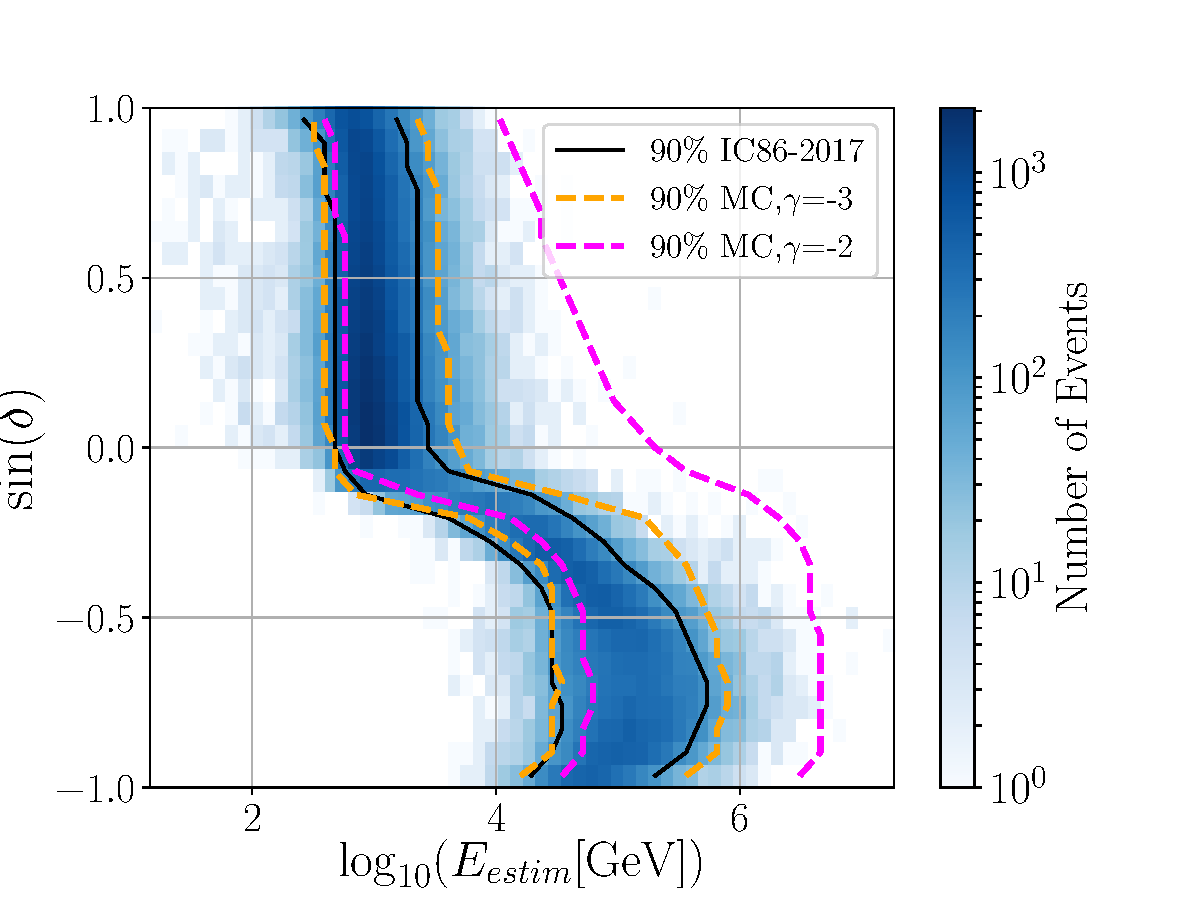
\includegraphics[width=\linewidth,viewport= 0 0 530 390, clip=true]{IC86II_enDist.pdf}
\caption[]{The distribution of events in one year of data for the final event selection as a function of reconstructed declination and estimated energy. The 90\% energy range for the data (black), as well as simulated astrophysical signal Monte-Carlo (MC) for an $E^{-2}$ and an $E^{-3}$ spectrum are shown in magenta and orange respectively as a guide for the relevant energy range of IceCube (from Ref.~\cite{Aartsen:2019fau}).}\label{fig:enDist}
\end{figure}
%%%%%%%%%%%%%%%%%

\section{Event Selection}\label{secII}

The {\tt PSTracks} event selection identifies high-energy muons passing through the IceCube detector with a goal of identifying sources of astrophysical neutrinos. The selection applies differing criteria in the Northern and Southern hemisphere -- corresponding to events originating below (``up-going'') and above (``down-going'') the IceCube detector, respectively -- with different atmospheric backgrounds. The boundary between the hemispheres is at declination $\delta=-5^\circ$, which is identical to a zenith angle of $95^\circ$ for the special location of IceCube. 

In the Northern hemisphere, atmospheric muons are filtered by the Earth. While some atmospheric muons are erroneously reconstructed into the Northern sky, the misreconstructed events can be removed by selecting high-quality track-like events. 

In the Southern hemisphere, the atmospheric background is reduced by strict cuts on the reconstruction quality and minimum energy, since the astrophysical neutrino fluxes are expected to have a harder energy spectrum than the background of atmospheric muons and neutrinos. 

%%%%%%%%%%%%%%%%%
%\begin{figure*}[t]
%\centering
%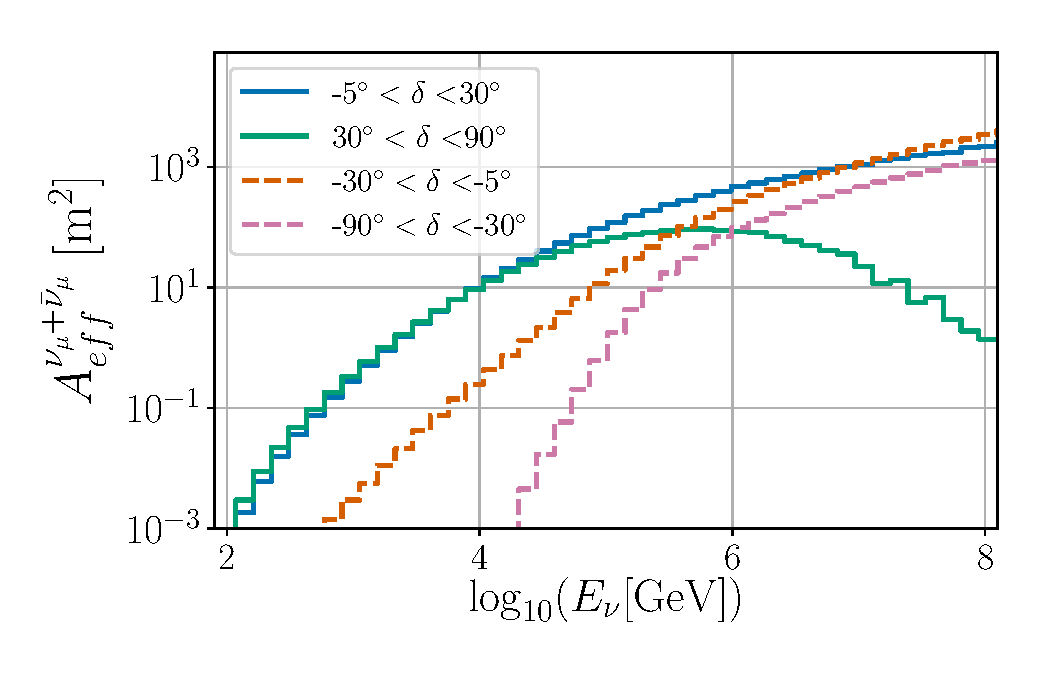
\includegraphics[width=0.51\linewidth,viewport= 20 20 500 330, %clip=true]{IC86II_effA.pdf}\hfill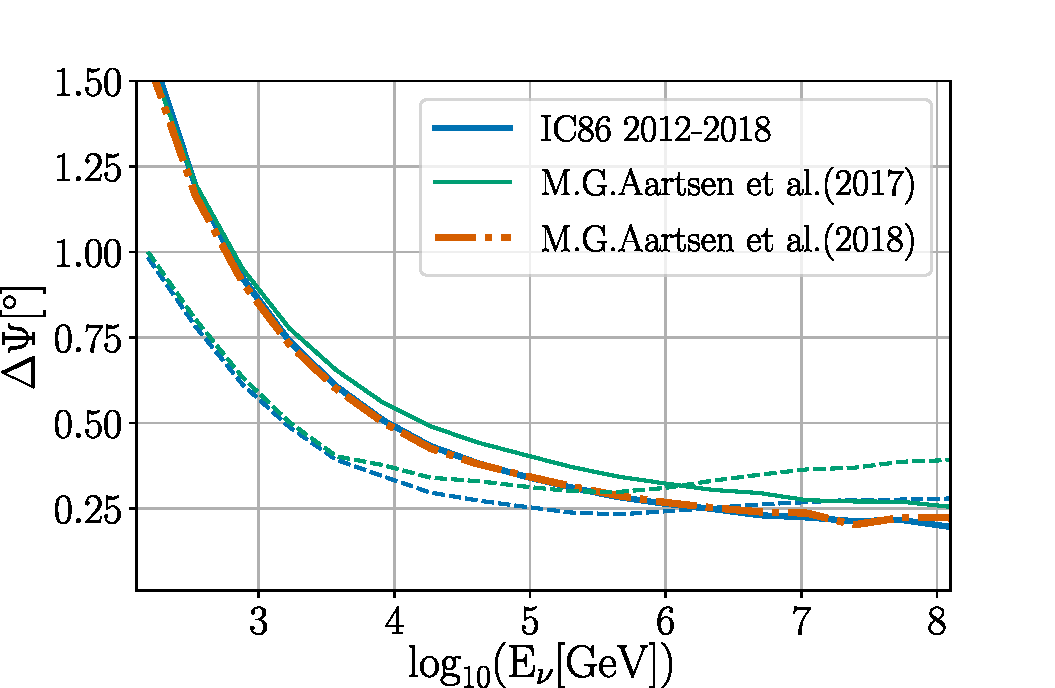
\includegraphics[width=0.48\linewidth,viewport= 0 0 480 310, %clip=true]{IC86II_PSF.pdf}
%\caption[]{{\bf Left:} The effective area as a function of neutrino energy for the IC86-II-VII %event selection averaged across the declination band for several declination bins using simulated %data. {\bf Right:} The median angle between simulated neutrino and reconstructed muon directions %as a function of energy. (Figures from Ref.~\cite{Aartsen:2019fau})}\label{fig:effAand PSF}
%\end{figure*}
%%%%%%%%%%%%%%%%%

%%%%%%%%%%%%%%%%%
%\begin{figure*}[t]
%\centering
%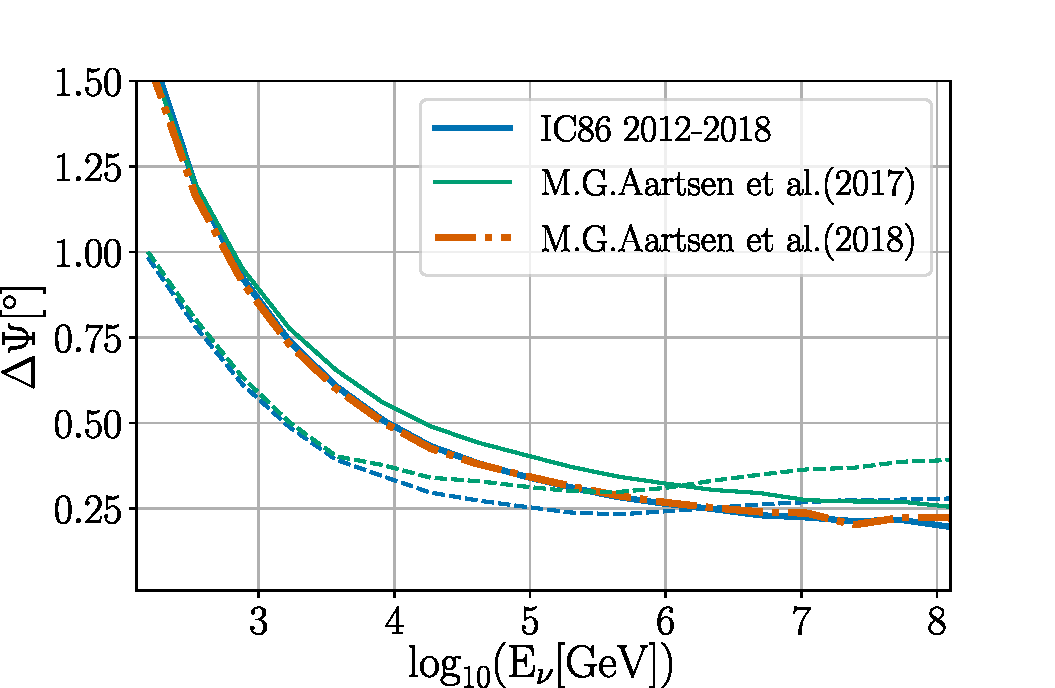
\includegraphics[width=0.48\linewidth,clip=true]{IC86II_PSF.pdf}
%\caption[]{The median angle between simulated neutrino and %reconstructed muon directions 
%as a function of energy. (Figures from %Ref.~\cite{Aartsen:2019fau})}\label{fig:PSF}
%\end{figure*}
%%%%%%%%%%%%%%%%%


%%%%%%%%%%%%%%%%%
\begin{figure*}[t]\centering
\begin{minipage}[c][6.5cm][c]{0.49\textwidth}\centering
{(a)}\\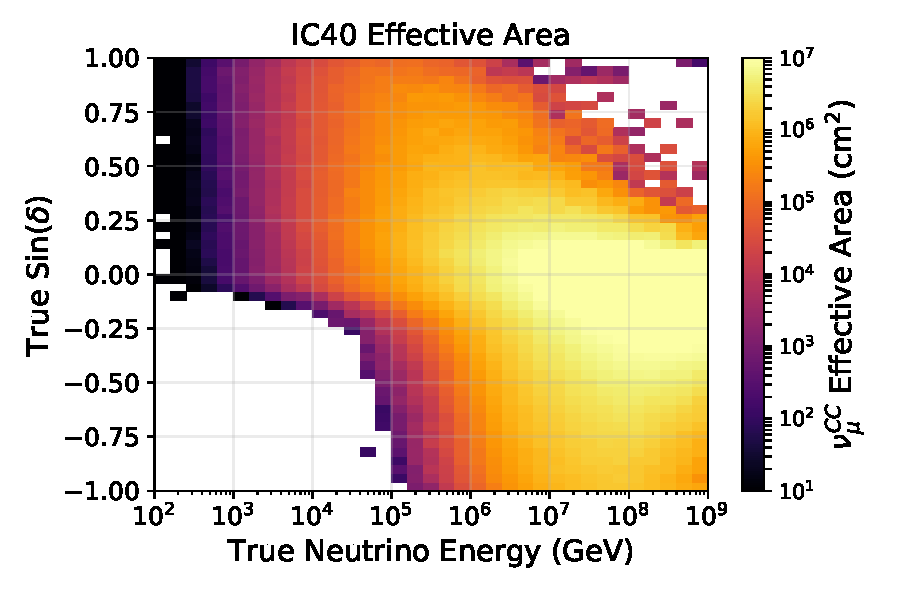
\includegraphics[width=\linewidth]{./PublicReleasePlots/EffectiveAreaPlots/IC40_effectiveArea.pdf}
\end{minipage}
\begin{minipage}[c][6.5cm][c]{0.49\textwidth}\centering
{(b)}\\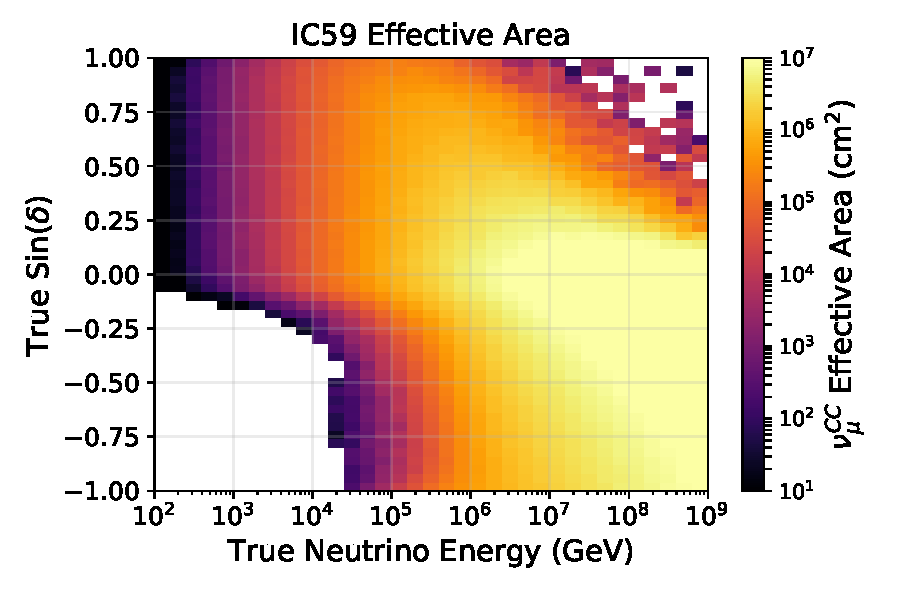
\includegraphics[width=\linewidth]{./PublicReleasePlots/EffectiveAreaPlots/IC59_effectiveArea.pdf}
\end{minipage}\\
\begin{minipage}[c][6.5cm][c]{0.49\textwidth}\centering
{(c)}\\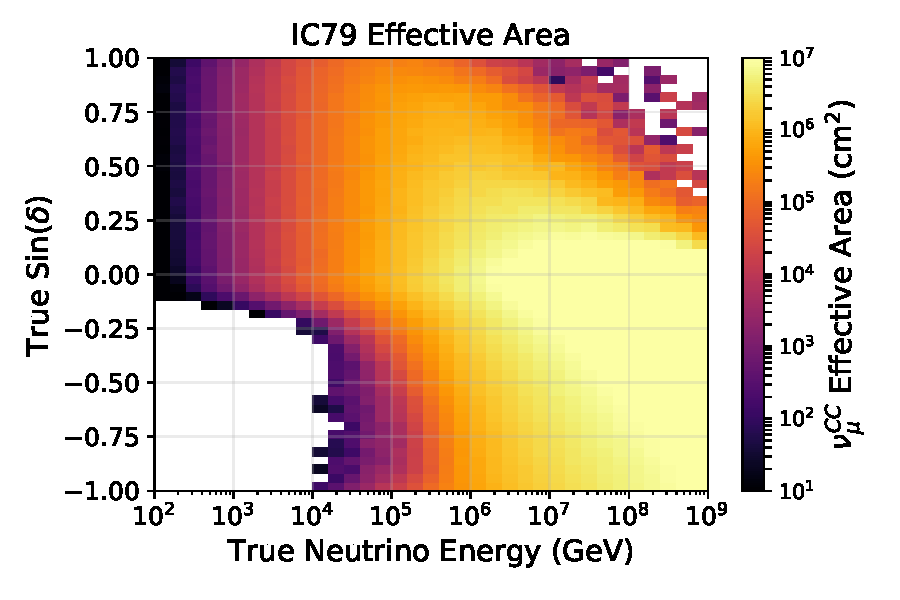
\includegraphics[width=\linewidth]{./PublicReleasePlots/EffectiveAreaPlots/IC79_effectiveArea.pdf}
\end{minipage}
\begin{minipage}[c][6.5cm][c]{0.49\textwidth}\centering
{(d)}\\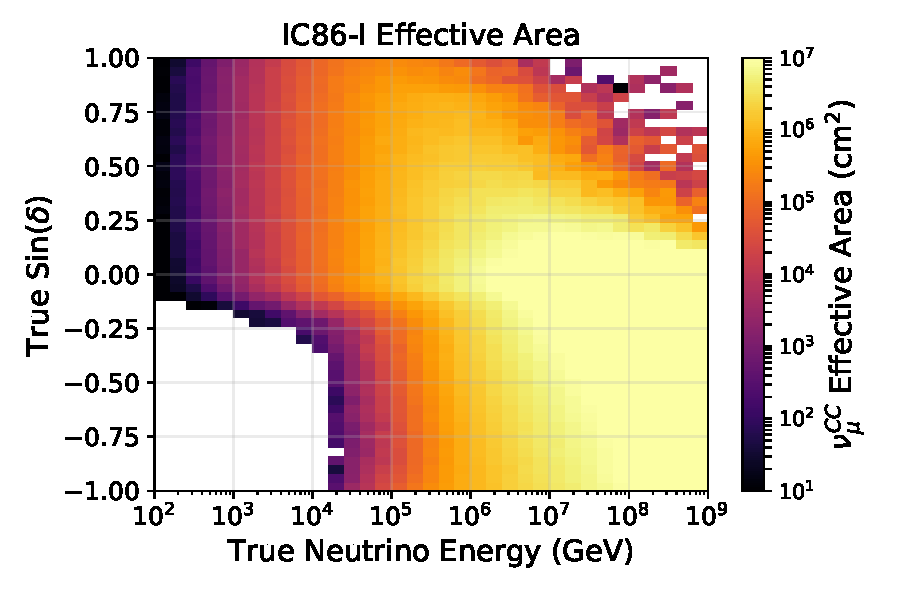
\includegraphics[width=\linewidth]{./PublicReleasePlots/EffectiveAreaPlots/IC86_I_effectiveArea.pdf}
\end{minipage}\\
\begin{minipage}[c][6.5cm][c]{0.49\textwidth}\centering
{(e)}\\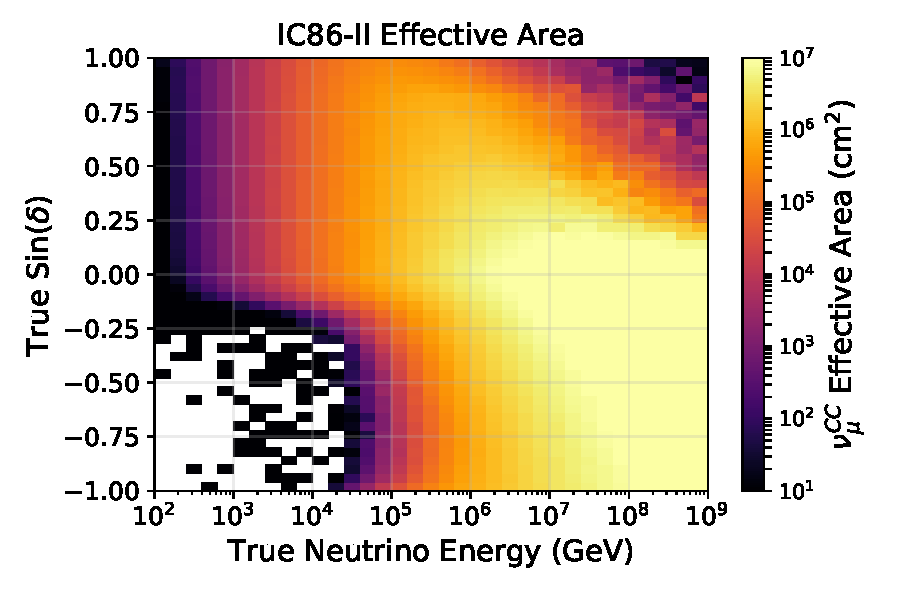
\includegraphics[width=\linewidth]{./PublicReleasePlots/EffectiveAreaPlots/IC86_II_effectiveArea.pdf}
\end{minipage}

\caption{The effective areas for each uniform data-taking period included in the current data release. IC40 through IC79 used the partially-completed detector while IC86-I and later followed detector completion. Software and calibration differences separate IC86-I from later years. Differences in the tools and applied selection have a small, but important impact on the sample for each period.}\label{fig:effA}
\end{figure*}
%%%%%%%%%%%%%%%%%

%%%%%%%%%%%%%%%%%
\begin{figure*}[t]\centering
\begin{minipage}[c][3.5cm][c]{0.30\textwidth}\centering
{(a)}\\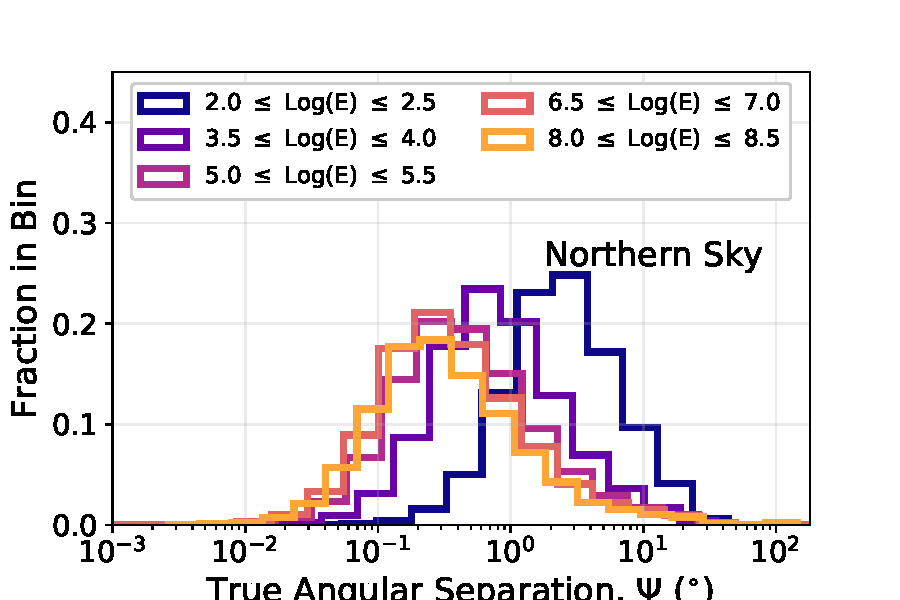
\includegraphics[width=\linewidth]{./PublicReleasePlots/ReconstructionPlots/IC86-II/IC86_II_MC_psf_2.pdf}
\end{minipage}
\begin{minipage}[c][3.5cm][c]{0.30\textwidth}\centering
{(b)}\\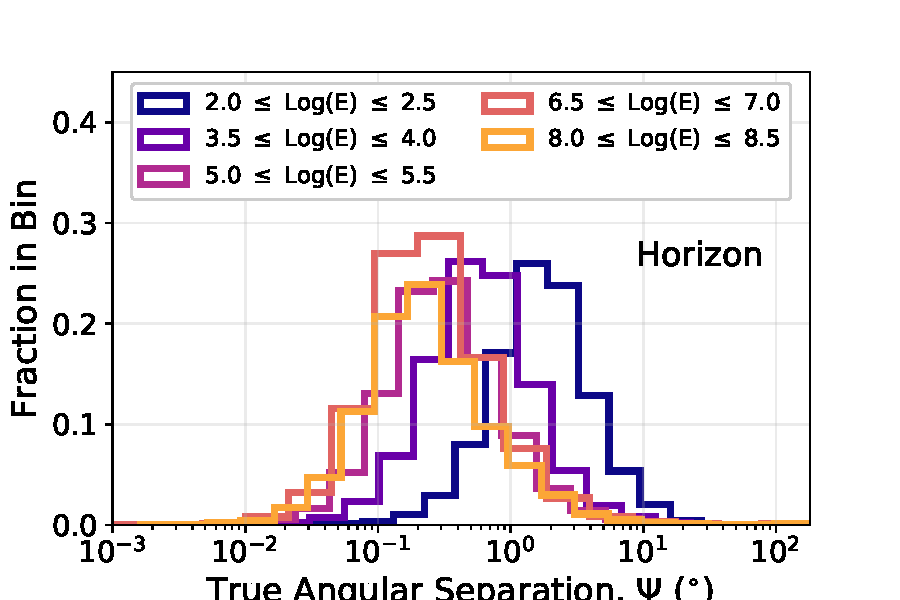
\includegraphics[width=\linewidth]{./PublicReleasePlots/ReconstructionPlots/IC86-II/IC86_II_MC_psf_1.pdf}
\end{minipage}
\begin{minipage}[c][3.5cm][c]{0.30\textwidth}\centering
{(c)}\\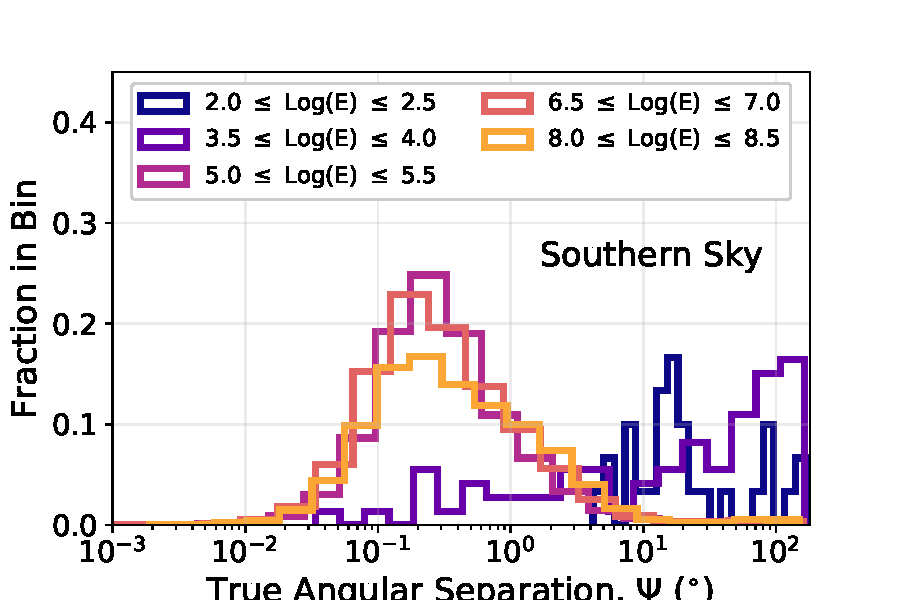
\includegraphics[width=\linewidth]{./PublicReleasePlots/ReconstructionPlots/IC86-II/IC86_II_MC_psf_0.pdf}
\end{minipage}
\caption{The binned point spread functions measured for the Northern sky ($\delta<-10^\circ$), horizon ($-10^\circ\leq\delta<-10^\circ$), and Southern sky ($\delta\geq 10^\circ$) for IC86-II and later seasons. Each colored histogram corresponds to a different true neutrino energy range. For a falling $E^{-2}$ spectrum, most muons are reconstructed less than 1$^\circ$ from the neutrino origin.}\label{fig:PSF}
\end{figure*}
%%%%%%%%%%%%%%%%%

%%%%%%%%%%%%%%%%%
\begin{figure*}[t]\centering
\begin{minipage}[c][3.5cm][c]{0.30\textwidth}\centering
{(a)}\\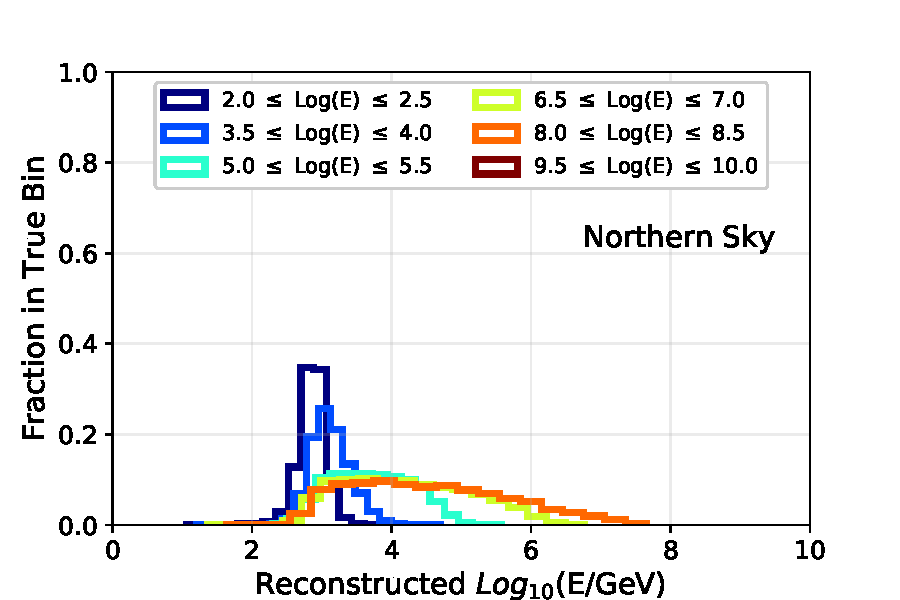
\includegraphics[width=\linewidth]{./PublicReleasePlots/ReconstructionPlots/IC86-II/IC86_II_MC_esmearing_2.pdf}
\end{minipage}
\begin{minipage}[c][3.5cm][c]{0.30\textwidth}\centering
{(b)}\\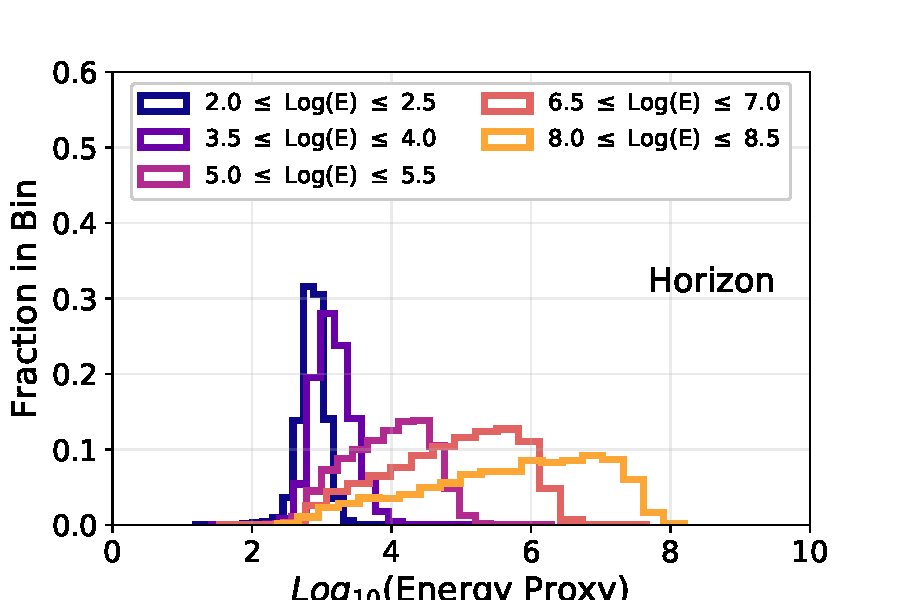
\includegraphics[width=\linewidth]{./PublicReleasePlots/ReconstructionPlots/IC86-II/IC86_II_MC_esmearing_1.pdf}
\end{minipage}
\begin{minipage}[c][3.5cm][c]{0.30\textwidth}\centering
{(c)}\\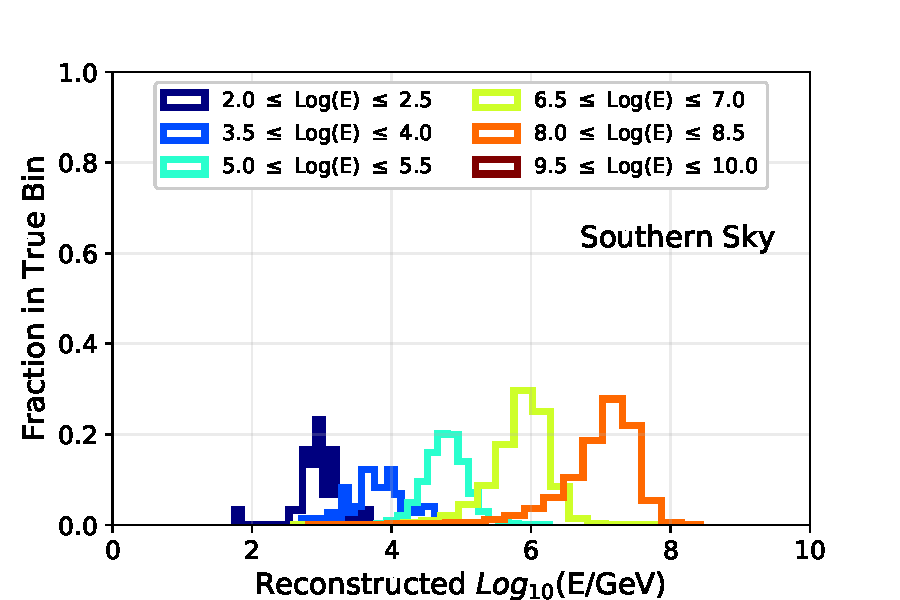
\includegraphics[width=\linewidth]{./PublicReleasePlots/ReconstructionPlots/IC86-II/IC86_II_MC_esmearing_0.pdf}
\end{minipage}
\caption{The binned muon energy proxy reconstruction measured for the Northern sky ($\delta<-10^\circ$), horizon ($-10^\circ\leq\delta<-10^\circ$), and Southern sky ($\delta\geq 10^\circ$) for IC86-II and later seasons. Each colored histogram corresponds to a different true neutrino energy range. In the Southern sky, high energy events reconstruct near the incident neutrino energy. In the Northern sky and at the horizon, high energy events may interact far from the detector, producing energy losses which are not visible in IceCube. }\label{fig:ESmearing}
\end{figure*}
%%%%%%%%%%%%%%%%%

%%%%%%%%%%%%%%%%%
\begin{figure*}[t]\centering
\begin{minipage}[c][3.5cm][c]{0.30\textwidth}\centering
{(a)}\\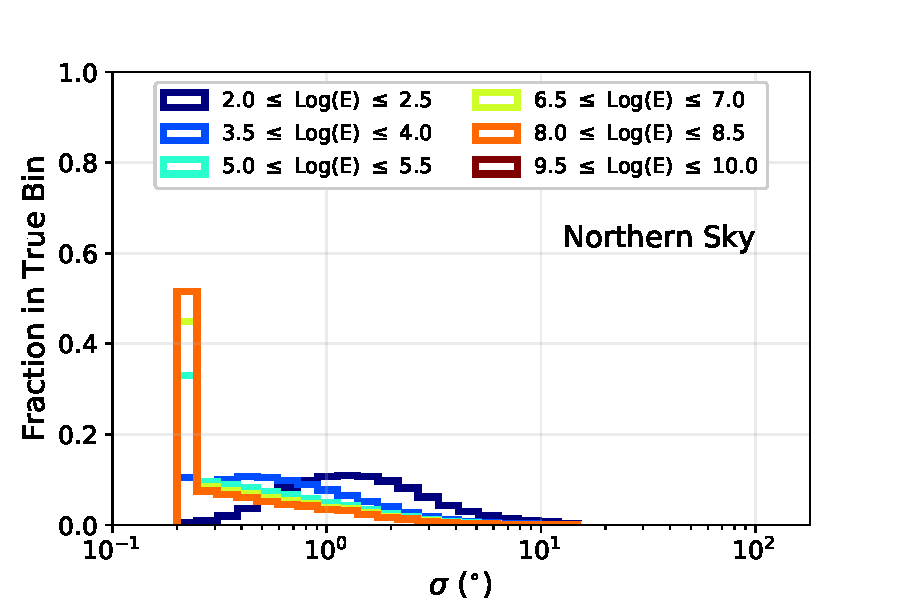
\includegraphics[width=\linewidth]{./PublicReleasePlots/ReconstructionPlots/IC86-II/IC86_II_MC_angErr_2.pdf}
\end{minipage}
\begin{minipage}[c][3.5cm][c]{0.30\textwidth}\centering
{(b)}\\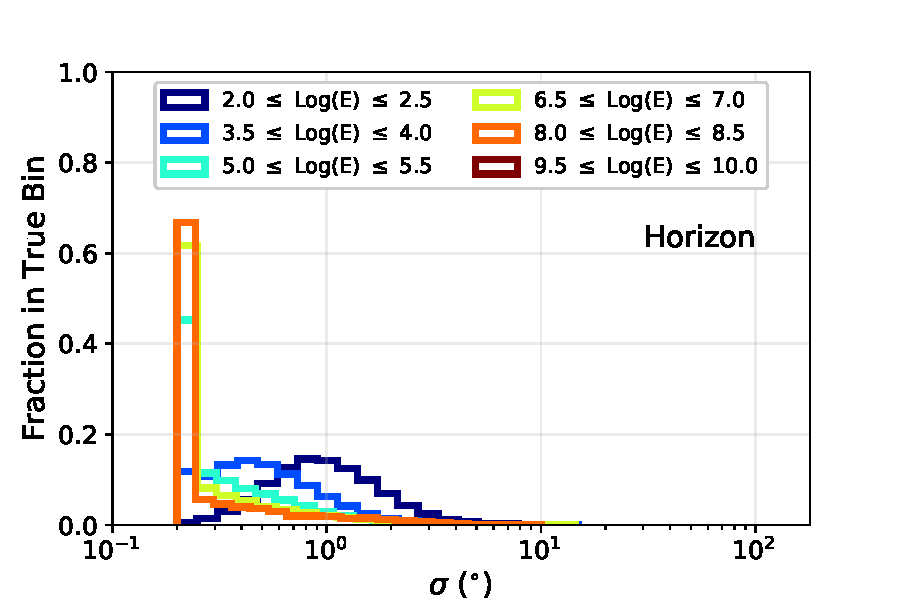
\includegraphics[width=\linewidth]{./PublicReleasePlots/ReconstructionPlots/IC86-II/IC86_II_MC_angErr_1.pdf}
\end{minipage}
\begin{minipage}[c][3.5cm][c]{0.30\textwidth}\centering
{(c)}\\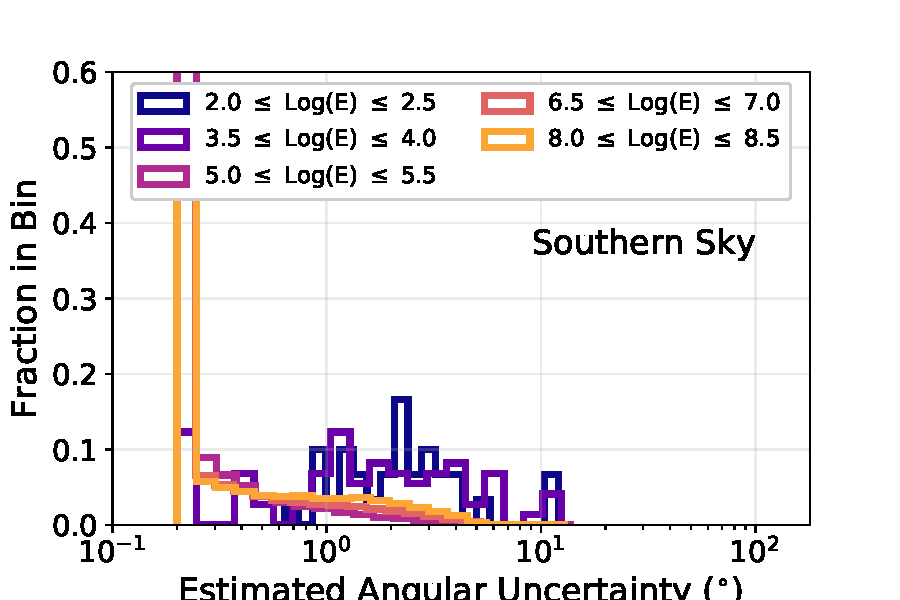
\includegraphics[width=\linewidth]{./PublicReleasePlots/ReconstructionPlots/IC86-II/IC86_II_MC_angErr_0.pdf}
\end{minipage}
\caption{The binned estimated angular uncertainty on the  reconstructed direction measured for the Northern sky ($\delta<-10^\circ$), horizon ($-10^\circ\leq\delta<-10^\circ$), and Southern sky ($\delta\geq 10^\circ$) for IC86-II and later seasons. Each colored histogram corresponds to a different true neutrino energy range. The estimated angular uncertainties have been calibrated to give correct coverage for an $E^{-2}$ spectrum. In order to avoid unaccounted-for uncertainties and to ensure no single event dominates our likelihood, a floor of 0.2$^\circ$ is included for all events.}\label{fig:AngErr}
\end{figure*}
%%%%%%%%%%%%%%%%%




The main data seasons IC86-II to IC86-VII use multi-variate Boosted Decision Trees (BDT) to reduce the background of atmospheric muons and cascade events. In the Northern hemisphere, a single BDT is trained to recognize three classes of events: single muon tracks from atmospheric and astrophysical neutrinos, atmospheric muons, and cascades; neutrino-induced tracks are treated as signal. This BDT uses 11 variables related to event topology and reconstruction quality. The Northern BDT preserves $\sim90\%$ of the atmospheric neutrinos and $\sim0.1\%$ of the atmospheric muons from the initial selection of track-like events~\cite{Aartsen:2016oji,Aartsen:2018ywr,Aartsen:2019fau}. In the Southern hemisphere, BDTs are used to select only the best-reconstructed track-like events at the highest energies. In addition, the BDTs use four variables related to deposited energy along the track, as well as the light-arrival time of photons at the DOMs~\cite{Aartsen:2014cva,Aartsen:2016oji}. The large backgrounds of atmospheric muons and muon bundles require harsh cuts to reduce their rate significantly, resulting in an effective selection of only very high energy events. The selection effectively removes most Southern hemisphere events with an estimated energy below $\simeq10$~TeV; see Fig.~\ref{fig:enDist}. The IceTop surface array is used in addition as an active veto against coincident air-shower events for vertically down-going events~\cite{Aartsen:2013uuv}. The final all-sky event rate of about $4$~mHz is dominated by atmospheric muon neutrino interactions from the Northern hemisphere and by high-energy, well-reconstructed atmospheric muons in the Southern hemisphere. The preceding four years of data, collected with configurations IC40 through IC86-I, are handled exactly as in the past~\cite{Abbasi:2010rd,Aartsen:2013uuv,Schatto:2014kbj,Aartsen:2014cva}.


%%%%%%%%%%%%%%%%%%
%\begin{figure}[t]
%\centering
%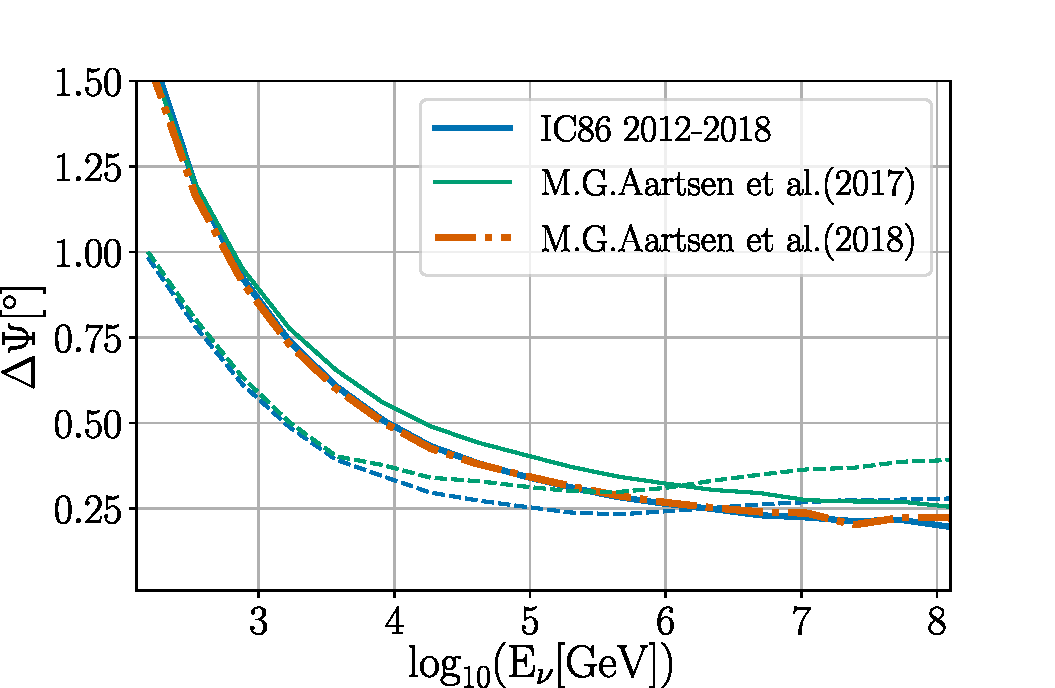
\includegraphics[width=\linewidth]{IC86II_PSF.pdf}
%\caption[]{\MA{\it (To be updated.)} The median angle between simulated neutrino and reconstructed muon directions as a function of energy (from Ref.~\cite{Aartsen:2019fau}).}\label{fig:PSF}
%\end{figure}
%%%%%%%%%%%%%%%%%%

\section{Detector Response}\label{secIII}

Muon tracks induced by astrophysical neutrino interactions are the main signal category in the search for point-like sources of neutrinos. Detailed Monte Carlo simulation is used to evaluate the response of IceCube to such events and distinguish them from atmospheric backgrounds. These simulations may be characterized by a combination of the effective areas ($A_\mathrm{eff}$) and the reconstruction response functions. 

The number of expected events $N_\nu$ is given by 
\begin{align}\label{eq:ev_rate}
N_\nu=\int dt \int d\Omega\int_0^\infty dE\,A_\mathrm{eff}\left(E, \Omega\right) \phi_\nu\left(E_\nu,\Omega, t\right)
\end{align}
The incident neutrino flux $\phi_\nu$ can have an assumed form or be derived from simulation; see \cite{Aartsen:2016xlq}. The effective area for each season varies as a function of neutrino energy and declination as shown in Figure~\ref{fig:effA}.

Reconstruction of events in {\tt PSTracks} proceeds in three steps, each incorporating effects from modeling of the Antarctic glacial ice medium. To begin, the direction of origin of the the candidate muon is reconstructed from the observed timing and charge in the detector following the algorithm described in Section~8.1 of ref~\cite{Ahrens:2004direc}. The angular distance between the reconstructed muon direction and the true neutrino direction is described by the point spread function (``PSF''). Binned examples of IceCube's PSF are shown in Figure~\ref{fig:PSF}.

The total energy loss of the muon track is then estimated following the description in ref~\cite{Aartsen:2014erec}. The energy reconstruction yields a proxy for the muon energy at detector entry and a lower limit on the candidate neutrino energy. The energy proxy can vary significantly for different declinations. For the Southern sky, observed muons from muon neutrino charged current interactions occur near the detector, giving an energy proxy close to the original neutrino's energy. For the Northern sky, neutrinos may interact while crossing the Earth before reaching IceCube, leading to unobservable energy losses, particularly at high energies. The energy proxy reconstruction is shown for IC86-II and later seasons in Figure~\ref{fig:ESmearing}.

The final stage is the estimation of the reconstruction angular uncertainty. The reconstruction likelihood space near the best-fit direction is mapped and fit with a paraboloid following ref~\cite{Neunhoeffer:2006}. The two dimensional width of the paraboloid fit is circularized by averaging the width across the two axes. In cases where the paraboloid method fails, {\tt PSTracks} instead relies on the Cramer-Rao method described in ref~\cite{Lunemann:2013oya}. In order to correct for the kinematic angle between neutrino and muon direction and to ensure correct coverage, a correction as a function of reconstructed energy is applied assuming an $E^{-2}$ flux such that the median estimated uncertainty as a function of energy gives 50\% containment for a two dimensional Gaussian distribution. While this correction can change with differing flux assumptions, the impact is small. A lower limit of 0.2$^\circ$ is applied to all events in order to avoid strong impacts from mismodeling of ice properties and to ensure that no single event dominates our likelihood calculations. The reconstruction angular uncertainties are shown in Figure~\ref{fig:AngErr}.

\section{Comparison to Previous Releases}\label{secIV}

There have been multiple previous IceCube data releases presenting track-like events in the Northern and Southern hemisphere, primarily for the purpose of neutrino astronomy ~\cite{Abbasi:2010rd,Aartsen:2013uuv,IceCube:2018,IceCube:2019,IceCube:TXS2018}. The dataset detailed in this document is the latest iteration of a sample of track-like events, with the goal of standardizing the IC86 II-VII data taking period. This dataset can be considered to be a successor of the previous data releases~\cite{IC40data,IC59data,IceCube:2018}, providing an updated description of the data from 2010--2012~\cite{IceCube:2018}, as well as adding six additional years of data in 2012--2018. 

This sample includes several improvements in addition to the aforementioned standardization of the IC86 data taking periods published in Ref.~\cite{IceCube:2018}. In this version of the data sample, the angular reconstruction has been improved, and the event classifier and sample pre-cuts have been altered to better reject cascade-like events and accept track-like events. 

The net effect of the sample changes is an increase in event rate ($\sim$7\%) relative to previous versions of the sample. A year-by-year comparison of event counts between the older \MA{({\tt PSTracks v2})} and newer \MA{({\tt PSTracks v3})} versions of this sample can be seen in Table~\ref{tab:v2v3evtcontent}. A comparison of the one-year time-integrated sensitivity for the IC86-IV season for the two samples can be seen in Figure~\ref{fig:v2v3senscompare}.

As an example of how the changing content of the different versions of this data sample can affect the process of searching for hotspots in IceCube data, we examine the 2014/2015 neutrino flare associated with TXS 0506+056~\cite{IceCube:2018cha}. The $3.5 \sigma$ excess seen in 2014/2015~\cite{IceCube:2018cha} was identified using the data sample corresponding to the data release ref. ~\cite{IceCube:2019}. Here, we repeat the untriggered flare search analysis, originally performed in ref. ~\cite{IceCube:2018cha}, but instead use the newest version of the data sample presented in this document, {\tt PSTracks v3}. The results of this cross-check can be seen in Table~\ref{tab:TXSCrossChecks}. Notably, the significance of the 2014/2015 neutrino flare decreases from $p=7.0 \times 10^{-5}$ ({\tt PSTracks v2}) to $p=8.1 \times 10^{-3}$ ({\tt PSTracks v3}) when using the most recent version of the data sample. A comparison of the reconstructed parameters of the most signal-like neutrino events contributing to the 2014/2015 flare in both versions of the data sample can be seen in Table~\ref{tab:TXSFlareEvtsTable} and Figure~\ref{fig:TXSEvtsCompare}.

The lower significance of the 2014/2015 neutrino flare in the most recent version of the sample has mainly been caused by the absence of two cascade-like events, occurring at MJD=56992.1586 and MJD=57014.1910, that existed in the {\tt PSTracks v2} data sample~\cite{IceCube:2019} associated with Ref.~\cite{IceCube:2018cha}, but have been removed from the {\tt PSTracks v3} data sample presented in this document. These two events did not pass a track length pre-cut that was introduced in the newest version of this data sample, requiring that all northern-sky events have a reconstructed track length greater than 200 meters. This pre-cut is intended to filter out poorly localized cascade events. Performing the untriggered flare search using {\tt PSTracks v2} (Ref.~\cite{IceCube:2019}) with the two cascade events manually removed results in a drop in significance similar to that which is observed when using {\tt PSTracks v3}, as seen in Table~\ref{tab:TXSCrossChecks}. The drop in significance cannot be otherwise adequately explained by changes to the angular reconstruction or other differences between the two versions of the sample. 

It should be noted that the apparent drop in significance of the 2014/2015 neutrino flare is not entirely unprecedented. A reduction in the time integrated pre-trials significance of TXS 0506+056 is also seen in Ref.~\cite{Aartsen:2019fau} when using the newer version of this sample: $p=2.0 \times 10^{-5}$~($4.1\sigma$) with \MA{\tt PSTracks v2} ~\cite{IceCube:2018cha}, and $p=1.9 \times 10^{-4}$~($3.5\sigma$) with \MA{\tt PSTracks v3} ~\cite{Aartsen:2019fau}. Note that these significances do not include corrections for the number of searches, as in Ref.~\cite{Aartsen:2019fau} and Ref~~\cite{IceCube:2018cha}.
 
 While both the time integrated and untriggered flare results associated with TXS 0506+056 appear to be less significant when using the newer version of this data sample, it is important to recognize that the results presented here are all \textit{a posteriori} cross checks preformed in order to explore the effects of the altered content of \MA{\tt PSTracks v3} in comparison to previous versions. While the two versions of the sample are very similar and have large overlaps, there is no reason a priori to prefer the \MA{\tt PSTracks v3} results over those of \MA{\tt PSTracks v2} and, as such, the previous result hold.
 The results of these checks are not intended to supersede the results shown in Ref.~\cite{IceCube:2018cha}.

%%%%%%%%%%%%%%%%%
\begin{figure*}[p]
\centering
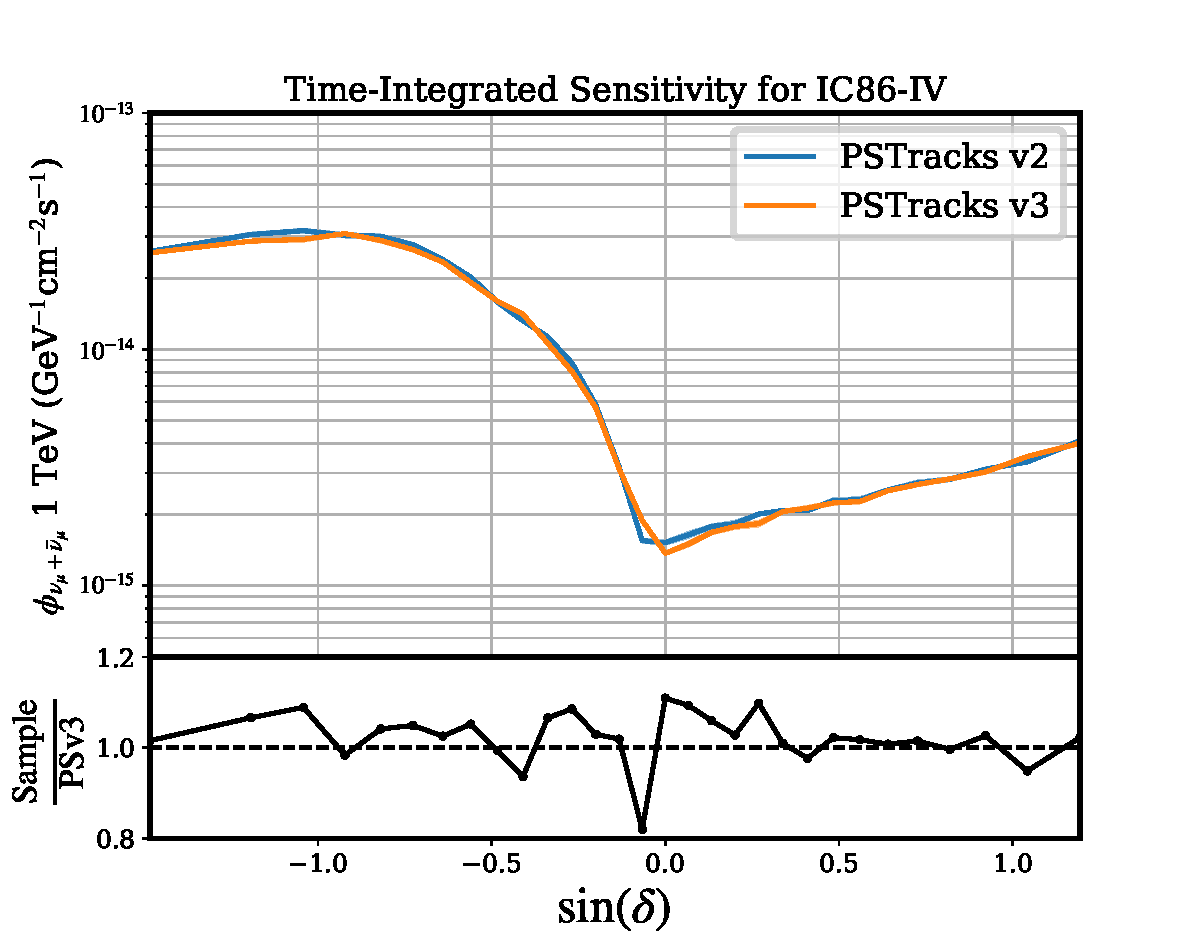
\includegraphics[width=0.5\linewidth,viewport= 0 0 530 390, clip=false]{./TXSCheckPlots/v2v3_senscompare.pdf}
\caption[]{A comparison of the 90\% C.L. sensitivity of a time-integrated point source search to an $E^{-2}$ source at various declinations. This is similar to the curves in figure 3 of Ref.~\cite{Aartsen:2019fau}, but here we calculate these values using only the IC86-IV season of both {\tt PSTracks v2} and {\tt PSTracks v3} for the purpose of comparing the two. For most declinations (particularly near the horizon), {\tt PSTracks v3} is a slight improvement over {\tt PSTracks v2}.}\label{fig:v2v3senscompare}
\end{figure*}
%%%%%%%%%%%%%%%%%

\begin{figure*}[p]
\centering
%\begin{minipage}{.5\textwidth}
%  \centering
%  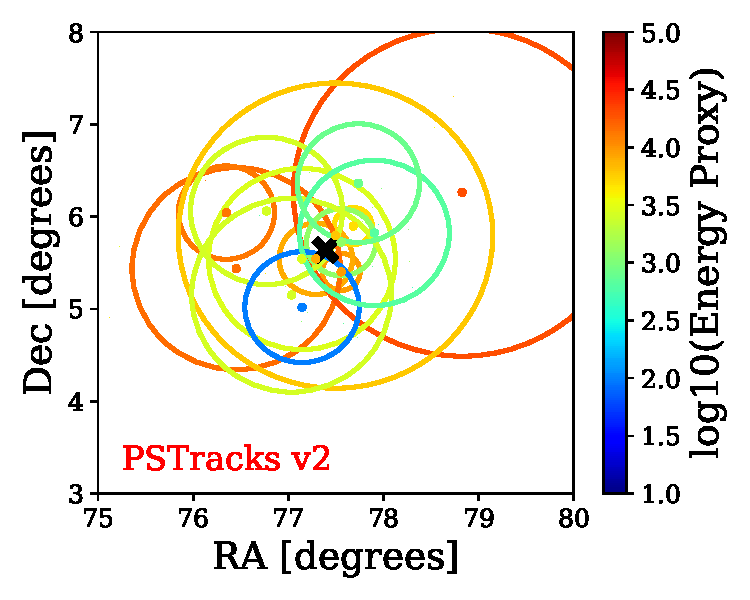
\includegraphics[width=.95\linewidth]{./TXSCheckPlots/PSTracksv2evtplot.pdf}
%  \label{fig:test1}
%\end{minipage}\hfill
%\begin{minipage}{.5\textwidth}
%  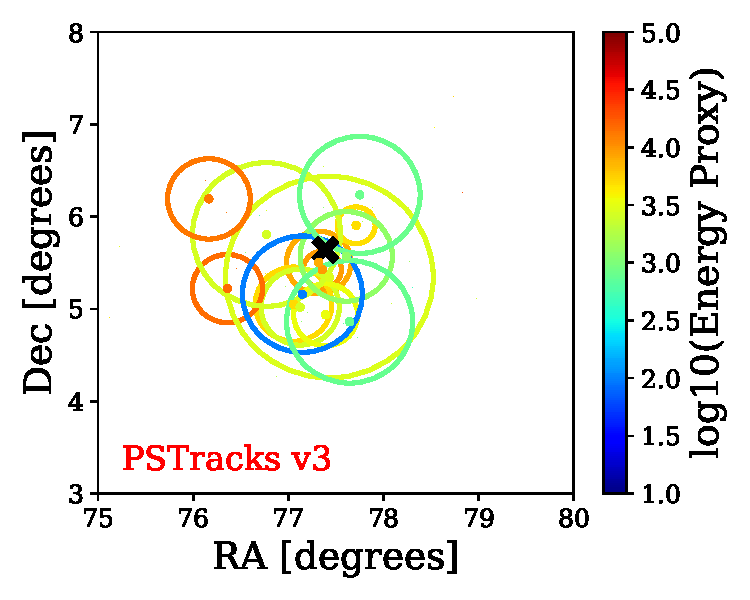
\includegraphics[width=.95\linewidth]{./TXSCheckPlots/PSTracksv3evtplot.pdf}
%  \label{fig:test2}
%\end{minipage}
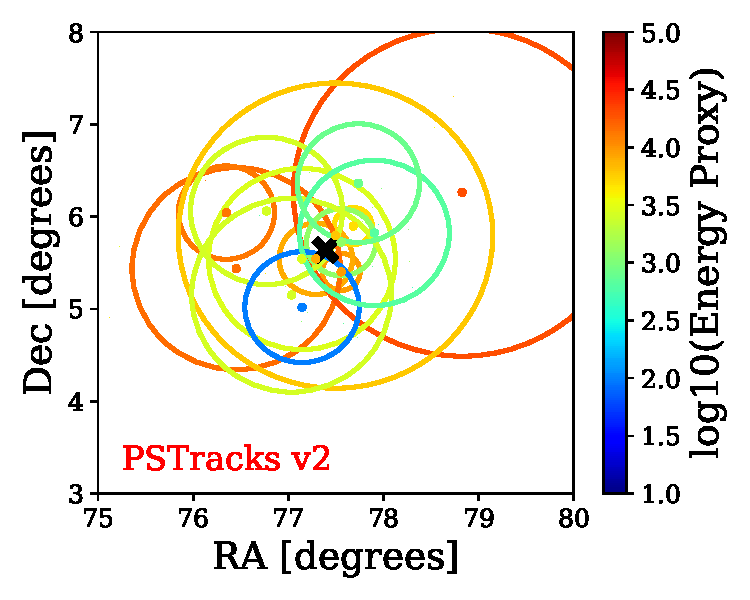
\includegraphics[width=.45\linewidth]{./TXSCheckPlots/PSTracksv2evtplot.pdf}\hspace{0.2in}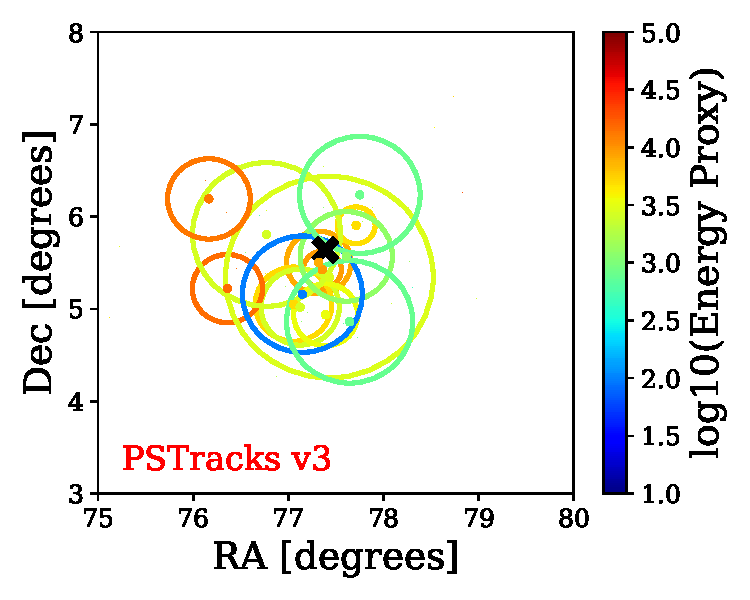
\includegraphics[width=.45\linewidth]{./TXSCheckPlots/PSTracksv3evtplot.pdf}
\caption[]{The top 14 most signal-like flare events contributing to the 2014/2015 neutrino flare associated with TXS 0506+056 (black ``$\times$''), both in \MA{\tt PSTracks v2} (left, used for the analysis published in Ref ~\cite{IceCube:2018cha}), and the updated sample presented in this document ({\tt PSTracks v3}, right). The size of the colored circles corresponds to the $1\sigma$ containment region of the angular reconstruction of that event, and the color of the circle corresponds to the reconstructed energy proxy.}\label{fig:TXSEvtsCompare}
\end{figure*}

\begin{table*}[p]
\centering
\begin{ruledtabular}
\begin{tabular}{lllccccc}
\multicolumn{8}{c}{Event Comparison Between \MA{\tt PSTracks~v2} and \MA{\tt PSTracks~v3}} \\[0.1cm]
Season & Start & End & Livetime & \MA{\tt PSTracks v2} & \MA{\tt PSTracks v3} & {\tt v2}$\rightarrow${\tt v3} Overlap & {\tt v3}$\rightarrow${\tt v2} Overlap \\ 
%IC40 & 2008/04/06 & 2009/05/20 & 376.4 & 36900 & 36900 & 100\% & 100\% \\
%IC59 & 2009/05/20 & 2010/05/31 & 352.6 & 107011 & 107011 & 100\% & 100\% \\
%IC79 & 2010/06/01 & 2011/05/13 & 316.0 & 93133 & 93133 & 100\% & 100\% \\
%IC86-I & 2011/05/13 & 2012/05/15 & 332.9 & 136244 & 136244 & 100\% & 100\% \\
IC86-II & 2012/04/26\footnotemark & 2013/05/02 & 332.0d & 105300 & 112858 & 88.0\% & 82.1\% \\
IC86-III & 2013/05/02 & 2014/05/06 & 362.9d & 114834 & 122541 & 87.8\% & 82.3\% \\
IC86-IV & 2014/04/10\footnotemark & 2015/05/18 & 370.7d & 118456 & 127045 & 87.9\% & 82.0\% \\
%IC86-V & 2015/04/24\footnotemark & 2016/05/20 & 365.4 & - & 129312 & - & - \\
%IC86-VI & 2016/05/20 & 2017/05/18 & 357.3 & - & 123657 & - & - \\
%IC86-VII & 2017/05/18 & 2018/07/08 & 410.6 & - & 145750 & - & - \\
\end{tabular}
\footnotetext[1]{Start date for test runs of the new processing. The remainder of this season began 2012/05/15}
\footnotetext[2]{Start date for test runs of the new processing. The remainder of this season began 2014/05/06}
%\footnotetext[3]{Start date for test runs of the new processing. The remainder of this season began 2015/05/18}
\end{ruledtabular}
\caption[]{A comparison of the sample content between \MA{\tt PSTracks v2} and \MA{\tt PSTracks v3} for the period of overlap between the two samples. The rightmost two columns report the overlap in event content between the old and new versions of the samples for periods of shared livetime. \MA{The entry ``{\tt v2}$\rightarrow${\tt v3}''} refers to the percentage of events in {\tt PSTracks v2} that are also in \MA{\tt PSTracks v3}, and \MA{``{\tt v3}$\rightarrow${\tt v2}''} is the reverse. The \MA{older} version ({\tt v2}) of the sample has been discontinued as of the IC86-2015 season, having been replaced by \MA{\tt PSTracks v3}. Seasons prior to IC86-II are identical between the two versions of the sample, and seasons after IC86-IV only exist in the \MA{newer} ({\tt v3}) version of the sample.}\label{tab:v2v3evtcontent}
\end{table*}

\begin{table*}[p]
\centering
\begin{ruledtabular}
\begin{tabular}{cccccc}
\multicolumn{6}{c}{Untriggered Flare Cross-check Results} \\[0.1cm]
Sample & p-value (pre-trial) & $T_\text{start}$ & $T_\text{stop}$ & $n_s$ & $\gamma$ \\ 
\MA{\tt PSTracks v2}~\cite{IceCube:2018cha,IceCube:2019} & 7.0e-5 & 56937.81 & 57096.22 & 14.39 & 2.20  \\
\MA{\tt PSTracks v2} w/o cascades & 1.17e-3 & 56937.81 & 57112.65 & 12.22 & 2.26 \\
\MA{\tt PSTracks v3} (this release) & 8.14e-3 & 56927.86 & 57116.76 & 11.87 & 2.22\\
\end{tabular}
\end{ruledtabular}
\caption[]{The results of repeating the untriggered flare analysis preformed in ~\cite{IceCube:2018cha}, but using {\tt PSTracks v3} in place of {\tt PSTracks v2} ~\cite{IceCube:2019}, the dataset that was originally used. The apparent drop in significance when using {\tt PSTracks v3} can be explained by cascade-like events present in {\tt v2} that have been removed from {\tt v3}.}\label{tab:TXSCrossChecks}
\end{table*}

\begin{table*}[p]
\centering
\begin{ruledtabular}
\begin{tabular}{c|cccc|cccc}
\multicolumn{9}{c}{Events Contributing to the 2014 TXS 0506+056 Neutrino Flare} \\[0.1cm]
\hline
\multicolumn{1}{c|}{} &
\multicolumn{4}{c|}{\MA{\tt PSTracks v2}~\cite{IceCube:2018cha,IceCube:2019}} & 
\multicolumn{4}{c}{\MA{\tt PSTracks v3} (this release)}\\[0.1cm]
MJD & RA (deg) & Dec (deg) & $\sigma$ (deg) & $\log_{10}(E/{\rm GeV})$ & RA (deg) & Dec (deg) & $\sigma$ (deg) & $\log_{10}(E/{\rm GeV})$\\ 
\hline
56940.9084 & 77.55 & 5.40 & 0.20 & 3.97 & 77.35 & 5.42 & 0.20 & 3.97\\
57009.5301 & 77.28 & 5.54 & 0.38 & 3.91 & 77.32 & 5.50 & 0.34 & 3.91\\
57089.4395 & 77.68 & 5.89 & 0.20 & 3.69 & 77.71 & 5.90 & 0.20 & 3.69\\
57072.9895 & 76.45 & 5.43 & 1.09 & 4.17 & 76.35 & 5.22 & 0.36 & 4.71\\
56992.1586 & 78.82 & 6.26 & 1.77 & 4.30 & - & - & - & - \\
56981.1313& 76.34 & 6.04 & 0.50 & 4.13 & 76.16 & 6.19 & 0.43 & 4.13 \\
56955.7917 & 77.55 & 5.72 & 0.36 & 3.09 & 77.60 & 5.56 & 0.48 & 3.0 \\
57014.1910 & 77.49 & 5.79 & 1.65 & 3.79 & - & - & - & -  \\
57112.6530 & 77.14 & 5.54 & 0.98 & 3.46 & 77.43 & 5.34 & 1.09 & 3.46 \\
56991.9383 & 76.77 & 6.06 & 0.79 & 3.42 & 76.77 & 5.80 & 0.77 & 3.42 \\
57072.2089 & 77.03 & 5.14 & 1.05 & 3.43 & 76.35 & 5.22 & 0.36 & 4.17 \\
56990.4325 & 77.14 & 5.01 & 0.60 & 1.99 & 77.14 & 5.15 & 0.63 & 1.99 \\
56940.5215 & 77.90 & 5.82 & 0.78 & 2.82 & - & - & - & - \\
56937.8190 & 77.73 & 6.36 & 0.64 & 2.91 & 77.75 & 6.23 & 0.63 & 2.91 \\
56973.3971 & - & - & - & - & 77.05 & 5.05 & 0.40 & 3.71 \\
56927.8601 & - & - & - & - & 77.39 & 4.93 & 0.33 & 3.53 \\
\end{tabular}
\end{ruledtabular}
\caption[]{The most signal-like events contributing to the 2014/2015 TXS 0506+056 neutrino flare in, both, the data sample published in Ref.~\cite{IceCube:2019} ({\tt PSTracks v2}) as well as the data sample presented here ({\tt PSTracks v3}). There were no changes to energy reconstruction between the two sample versions, but the angular reconstruction and sample event content have changed. The events occurring at MJD=56992.1586 and MJD=57014.1910 are cascade events that have been treated as tracks by the reconstruction, and as such the direction and energy information reported in the {\tt PSTracks v2} sample is unlikely to be a good description of the true event properties.}\label{tab:TXSFlareEvtsTable}
\end{table*}

\begin{acknowledgements}
\begin{center}\MA{(\it List of agencies in final version)}\end{center}
%USA {\textendash} U.S. National Science Foundation-Office of Polar Programs,
U.S. National Science Foundation-Physics Division,
Wisconsin Alumni Research Foundation,
Center for High Throughput Computing (CHTC) at the University of Wisconsin{\textendash}Madison,
Open Science Grid (OSG),
Extreme Science and Engineering Discovery Environment (XSEDE),
U.S. Department of Energy-National Energy Research Scientific Computing Center,
Particle astrophysics research computing center at the University of Maryland,
Institute for Cyber-Enabled Research at Michigan State University,
and Astroparticle physics computational facility at Marquette University;
Belgium {\textendash} Funds for Scientific Research (FRS-FNRS and FWO),
FWO Odysseus and Big Science programmes,
and Belgian Federal Science Policy Office (Belspo);
Germany {\textendash} Bundesministerium f{\"u}r Bildung und Forschung (BMBF),
Deutsche Forschungsgemeinschaft (DFG),
Helmholtz Alliance for Astroparticle Physics (HAP),
Initiative and Networking Fund of the Helmholtz Association,
Deutsches Elektronen Synchrotron (DESY),
and High Performance Computing cluster of the RWTH Aachen;
Sweden {\textendash} Swedish Research Council,
Swedish Polar Research Secretariat,
Swedish National Infrastructure for Computing (SNIC),
and Knut and Alice Wallenberg Foundation;
Australia {\textendash} Australian Research Council;
Canada {\textendash} Natural Sciences and Engineering Research Council of Canada,
Calcul Qu{\'e}bec, Compute Ontario, Canada Foundation for Innovation, WestGrid, and Compute Canada;
Denmark {\textendash} Villum Fonden, Danish National Research Foundation (DNRF), Carlsberg Foundation;
New Zealand {\textendash} Marsden Fund;
Japan {\textendash} Japan Society for Promotion of Science (JSPS)
and Institute for Global Prominent Research (IGPR) of Chiba University;
Korea {\textendash} National Research Foundation of Korea (NRF);
Switzerland {\textendash} Swiss National Science Foundation (SNSF);
United Kingdom {\textendash} Department of Physics, University of Oxford.
\end{acknowledgements}

\bibliographystyle{utphys_mod}

\bibliography{references}

\end{document}

